\documentclass[a4paper,14pt]{report} %размер бумаги устанавливаем А4, шрифт 12пунктов
\usepackage[T2A]{fontenc}
\usepackage[utf8]{inputenc}
\usepackage[english,russian]{babel} %используем русский и английский языки с переносами
\usepackage{amssymb,amsfonts,amsmath,mathtext,cite,enumerate,float} %подключаем нужные пакеты расширений
\usepackage[pdftex,unicode,colorlinks=true,linkcolor=blue]{hyperref}
\usepackage{indentfirst} % включить отступ у первого абзаца
\usepackage[dvips]{graphicx} %хотим вставлять рисунки?
\graphicspath{{illustr/}}%путь к рисункам

\makeatletter
\renewcommand{\@biblabel}[1]{#1.} % Заменяем библиографию с квадратных скобок на точку:
\makeatother %Смысл этих трёх строчек мне непонятен, но поверим "Запискам дебианщика"

\usepackage{geometry} % Меняем поля страницы. 
\geometry{left=1cm}% левое поле
\geometry{right=1cm}% правое поле
\geometry{top=1cm}% верхнее поле
\geometry{bottom=2cm}% нижнее поле

\renewcommand{\theenumi}{\arabic{enumi}}% Меняем везде перечисления на цифра.цифра
\renewcommand{\labelenumi}{\arabic{enumi}}% Меняем везде перечисления на цифра.цифра
\renewcommand{\theenumii}{.\arabic{enumii}}% Меняем везде перечисления на цифра.цифра
\renewcommand{\labelenumii}{\arabic{enumi}.\arabic{enumii}.}% Меняем везде перечисления на цифра.цифра
\renewcommand{\theenumiii}{.\arabic{enumiii}}% Меняем везде перечисления на цифра.цифра
\renewcommand{\labelenumiii}{\arabic{enumi}.\arabic{enumii}.\arabic{enumiii}.}% Меняем везде перечисления на цифра.цифра


\LARGE
\begin{document}
\newcommand{\pp}{Предположим противное}
%\newcommand{\pp}{{\LARП\!\!\!\!п~}}
\newcommand{\dokvo}{\paragraph{Доказательство.}}
\newcommand{\dokno}{\textbf {Доказано.}}
\newcommand{\neobh}{\paragraph{Необходимость.}}
\newcommand{\dost }{\paragraph{Достаточность.}}
\newcommand{\opred}{\paragraph{Определение.}}
\newcommand{\mnemo}{\paragraph{Мнемоника.}}
\newcommand{\N}{\mathbb{N}}
\newcommand{\Z}{\mathbb{Z}}
\newcommand{\Q}{\mathbb{Q}}
\newcommand{\R}{\mathbb{R}}
\renewcommand{\C}{\mathbb{C}}
\newcommand{\Beta}{B}%Костыль, а что поделать?
\newcommand{\Rn}{$\mathbb{R}^n~$}
\newcommand{\Rm}{$\mathbb{R}^m~$}
\renewcommand{\epsilon}{\varepsilon}
\renewcommand{\geq}{\geqslant}
\renewcommand{\leq}{\leqslant}
\newcommand{\fXR}{Пусть $X \subset \R, f:X \to \R$ }
\newcommand{\fXRx}{\fXR, $x_0$ - предельная точка $X$ }
\newcommand{\sgn}{\mathrm{sgn}~}
\newcommand{\nid}{\Leftrightarrow}
\newcommand{\intl}{\int\limits}
\newcommand{\Models}{|\!\!\!=\!\!\!|}
\newcommand{\Rightleftarrow}{\Leftrightarrow}

\newcommand{\xI}{{\vec{\xi}}}%Костыль для тервера, очень уж там часто встречается
\newcommand{\calF}{\mathcal{F}}
\newcommand{\calB}{\mathcal{B}}
\newcommand{\GOFP}{$G \sim \left<\Omega,\calF,P\right>$}

\newenvironment{zamena}[1][c]{=\left<\begin{array}{#1}}{\end{array}\right>=}

\newtheorem{theorem}{Теорема}[section]
\newenvironment{teorema}[1][{}]{\begin{theorem}{#1}\upshape}{\end{theorem}}

\theoremstyle{definition}

\newtheorem{zamech}{Замечание}[section]
\newtheorem{primer}{Пример}[section]
\newtheorem{opr}{Определение}[section]

\newtheorem{sledstvie}{Следствие}[theorem]
\newtheorem{utverzhd}[theorem]{Утверждение}
\newtheorem{lemma}[theorem]{Лемма}

\long\def\comment{}

\tableofcontents % это оглавление, которое генерируется автоматически
\LARGE

\chapter{Введение в анализ}
\section{Элементарные сведения из логики и теории множеств}
\subsection{Высказывания, предикаты связки}
\subsection{Кванторы}
\subsection{Множества, равенство двух множеств, подмножества}
\subsection{Простейшие операции над множествами}
\subsection{Принцип двойственности}
\subsection{Понятие счетного множества}
...

\section{Теория вещественных чисел}
\subsection{Множество рациональных чисел и его свойства}
\subsection{Вещественные числа, основные свойства вещественных чисел}
\subsection{Промежутки и их виды}
\subsection{Основные леммы теории вещественных чисел}
...

\section{Ограниченное множество, границы}
\subsection{Границы множества}
\subsection{Существование точной верхней границы у ограниченного сверху множества}
\subsection{Сечения в множестве рациональных чисел}
\subsection{Свойства $\sup$ и $\inf$}
\subsection{Отделимость множеств, лемма о системе вложенных отрезков}
\subsection{Лемма о последовательности стягивающихся отрезков}
...

\section{Отображения, функции}
\subsection{Отображения, виды отображений и т. д.}
\subsection{Вещественные функции}
...

\section{Предел последовательности}
\subsection{Последовательность элементов множества, числовая последовательность, определения предела числовой последовательноcти и бесконечно малой последовательности}
\subsection{Единственность предела последовательности}
\subsection{Подпоследовательности, связь пределов последовательности и подпоследовательности}
\subsection{Лемма о двух милиционерах}
\subsection{Основные теоремы о пределах последовательности}
\subsection{Понятие бесконечно большой последовательности}
\subsection{Монотонные последовательности, критерий существования предела монотонной послед}
\subsection{Существование предела последовательности $(1+1/n)^n$, число $e$ }
...

\section{Понятие предельной точки числового множества, теорема Больцано-Вейерштрасса, критерий Коши}
\subsection{Предельная точка множества}
\subsection{Теорема о последовательности, сходящейся к предельной точке}
\subsection{Теорема Больцано-Вейерштрасса}
\subsection{Критерий Коши}
...

\section{Верхний и нижний пределы последовательности}
\subsection{Понятие расширенной числовой прямой, понятие бесконечных пределов}
\subsection{Понятие частичных верхних и нижних пределов последовательности. Теорема о существовании у каждой последовательности ее верхнего и нижнего предела}
\subsection{Характеристические свойства верхнего и нижнего предела последовательности}
\subsection{Критерий существования предела последовательности}
...


\chapter{Вещественная функция вещественного аргумента}
\section{Предел вещественной функции вещественного аргумента}
\subsection{Определение предела функции по Коши, примеры}
\begin{opr}
	Число $b$ называется пределом функции $f(x)$ при $x$, стремящемся к $a$, если
	\begin{equation}
		\forall(\varepsilon > 0)\exists(\delta>0)\forall(x: 0<|x-a|<\delta)[|f(x)-b|<\varepsilon]
		.
	\end{equation}
	Пишут:
	\begin{equation}
		\lim_{x\to a} f(x) = b
		.
	\end{equation}
\end{opr}
Сама функция $f$ может и не быть определена в точке $a$, например
\begin{equation}
	\lim_{x\to 0} \frac{\sin x}{x} = 0
	,
\end{equation}

\begin{equation}
	\lim_{x\to 1} \frac{x^2-1}{x-1} = 2
	.
\end{equation}

Вообще говоря, предела у функции может и не существовать.
Например, не существует предела
\begin{equation}
	\lim_{x\to 0} \frac{|x|}{x}
	.
\end{equation}

\subsection{Определение предела функции по Гейне, примеры, эквивалентность определений}
\subsection{Обобщение понятия предела функции на расширенную числовую ось}
...

\section{Свойства пределов функции и функций, имеющих предел}
\subsection{Свойства, связанные с неравенствами}
\subsection{Свойства, связанные с арифметическими  операциями}
\subsection{Рецептурный подход к вычислению пределов}
Материал данного пункта относится скорее к практическим занятиям
и содержит указания о том, как вычислять пределы встречающихся на практике выражений.

\paragraph{Алгоритм действий при вычислении предела функции}
Пусть дан предел:
\begin{equation}
	\lim_{x\to a} f(x)
	,
\end{equation}
где $f(x)$ "--- <<достаточно хорошая>> функция.
Большинство встречающихся на практике функций <<достаточно хороши>>:
многочлены, степенные функции, тргонометрические функции и т.д.,
а также их сумма, разность, суперпозиция (например, $\sin (\ln x)$) и даже частное.

1. Попробуем вычислить $f(a)$.
Если это удалось "--- предел найден.
Но, как правило, это не удаётся по одной (или нескольким) из следующих причин:

а) Деление нуля на ноль. Пример:
\begin{equation}
	\lim_{x\to 1} \frac{x^2-1}{x-1}
	.
\end{equation}
В таком случае необходимо либо сокращать дробь <<вручную>> (для многочленов часто помогает схема Горнера при $x_0 = a$),
либо применять правило Лопиталя (см. ниже).


б) Деление ненулевого числа на ноль. Пример:
\begin{equation}
	\lim_{x\to 0} \frac{x^2+1}{x}
	.
\end{equation}
В таком случае возникает бесконечность. Пишут: $\infty$.

в) Деление бесконечности на бесконечность. Пример:
\begin{equation}
	\lim_{x\to \infty} \frac{x^2+1}{x^3+3}
	.
\end{equation}
Действия "--- как при делении нуля на ноль.
В нашем случае:
\begin{equation}
	\lim_{x\to \infty} \frac{x^2+1}{x^3+3}
	=
	\lim_{x\to \infty} \frac{x^{-1}+\frac1{x^3}}{1+\frac{3}{x^3}}
	=
	0
	.
\end{equation}

г) Вычитание бесконечности из бесконечности. Пример:
\begin{equation}
	\lim_{x\to \infty} \sqrt{2x-1} - \sqrt{x+1}
	.
\end{equation}
В ряде случаев помогает умножение на сопряжённое или вынос общего множителя за скобки.

д) Степенные неопределённости: $1^\infty$, $0^0$, $\infty^0$.
Пример (второй замечательный предел):
\begin{equation}
	\lim_{x \to \infty}\left(1 + \frac{1}{x}\right)^x =
	\lim_{x \to \infty}e^{x \cdot \ln\left(1 + \frac{1}{x}\right)} =
	e^{\lim_{x \to \infty} x \cdot \ln\left(1 + \frac{1}{x}\right)}
	e^{\lim_{x \to \infty} \frac{\ln\left(1 + \frac{1}{x}\right)}{1/x}}
\end{equation}
(дальнейшее может быть вычислено по правилу Лопиталя).
Обратим внимание читателя на следующие два приёма.
Во-первых, определение логарифма:
\begin{equation}
	a = e^{\ln a}, ~~\mbox{в частности,}~~  a^b = e^{b\cdot \ln a}
	.
\end{equation}
Во-вторых, функция $\exp(x)=e^x$ непрерывна и, следовательно, её можно менять местами со знаком предела:
\begin{equation}
	\lim_{x \to c} e^{f(x)} = e^{ \lim_{x \to c}f(x)}
	.
\end{equation}


\paragraph{Задачи для самостоятельного решения}
\begin{enumerate}
	\item
		\begin{equation}
			\lim_{x\to3}\frac{x^2-4}{x^2+x-6}
		\end{equation}
	\item
		\begin{equation}
			\lim_{x\to2}\frac{x^2-4}{x^2+x-6}
		\end{equation}
	\item
		\begin{equation}
			\lim_{x\to\infty}\frac{x^2+x^4}{x^3-x^2}
		\end{equation}
	\item
		\begin{equation}
			\lim_{x\to\infty}\frac{x^2+x^4}{x^5-x^2}
		\end{equation}
	\item
		\begin{equation}
	\lim_{x\to \infty} \sqrt{x-1} - \sqrt{x+1}
		\end{equation}
\end{enumerate}

...

\section{Односторонние пределы функции}
\subsection{Определение односторонних пределов, связь между существованием предела и односторонних пределов функции}
\subsection{Теорема о существовании односторонних пределов у монотонной функции и её следствия}
...

\section{Критерий Коши, замечательные пределы, бесконечно малые функции}
\subsection{Критерий Коши существования предела функции}
\subsection{Первый замечательный предел}
\opred
 $\lim\limits_{x\rightarrow 0} \frac{\sin(x)}{x}=1$

\subsubsection{Доказательство}
\begin{wrapfigure}{r}[5pt]{0.4\textwidth}
	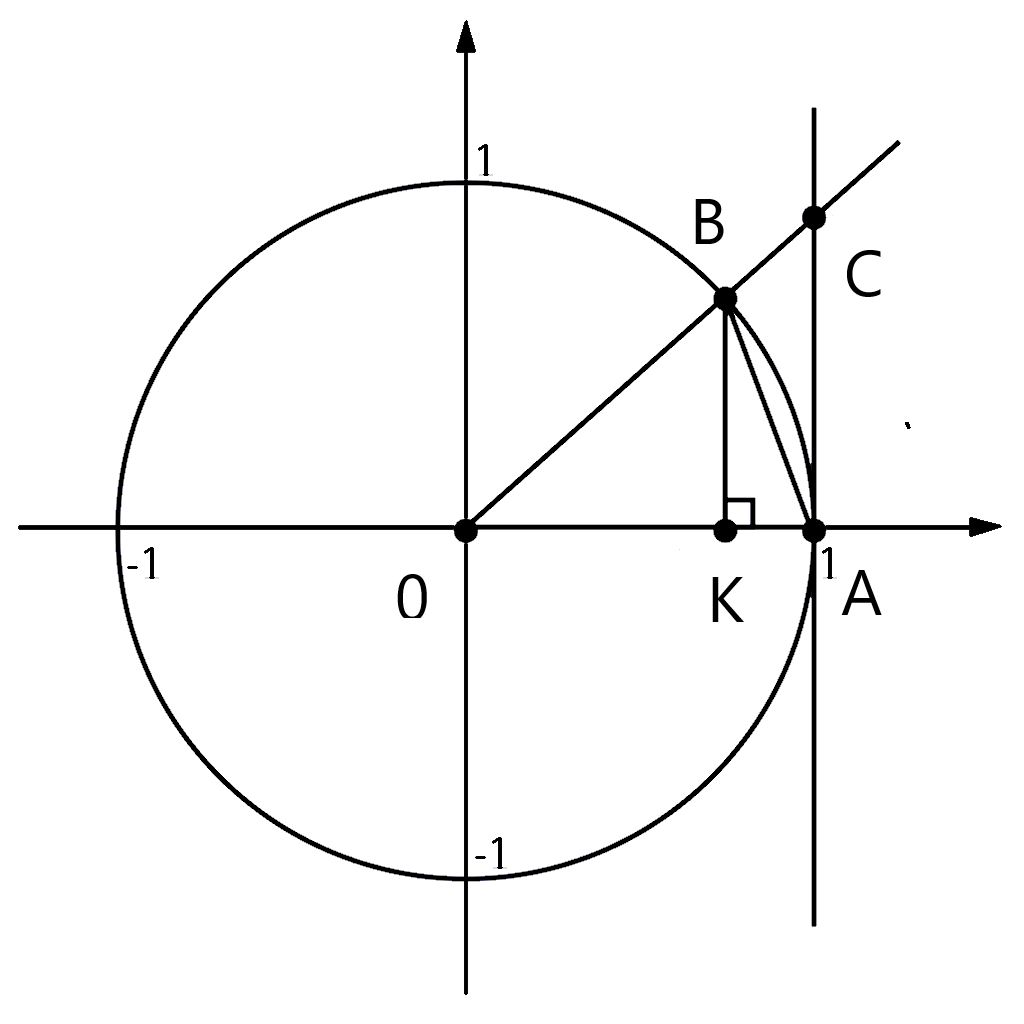
\includegraphics[scale=0.2]{image.png}
\end{wrapfigure}

Рассмотрим $\triangle$ DAB, $\triangle$ DAC и сектор OAB.
x-длинна дуги.
При $x \rightarrow 0$ их S уменьшаются.


$$ S\triangle{OBA} = \frac{1}{2}OA \cdot BK = \frac{\sin(x)}{2}$$
$$ S\triangle{OCA} = \frac{1}{2}OA \cdot AC = \frac{\operatorname{tg}(x)}{2}$$
$$ S(OBA) = \frac{1}{2}x \cdot r = \frac{x}{2}.$$

т.к. $ S\triangle OBA < SOBA < SOCA$
$\sin(x) < x < \operatorname{tg}(x)$

  $1  < \frac{x}{\sin(x)} < \frac{1}{\cos(x)}$

  $1 > \frac{\sin(x)}{x} > \cos(x)$

  это неравенство верно $\forall (x: 0 < |x|<\frac{\pi}{2})$.

  Функция, предел которой надо найти лежит между двумя функциями:
   $$\forall(\epsilon>0)\exists(\beta>0)\forall(x \in \mathbb{R})[0 < |x| <\beta \Rightarrow |\cos(x) - 1| < \epsilon]$$
  $$|\cos(x) - 1| = |2\sin^2(\frac{X}{2})| \leq 2|\sin\frac{x}{2}| < \frac{2|x|}{2} = |x| < \epsilon.$$

  Мы нашли $\beta : \beta = \epsilon$, т.к. |x| < $\beta$ и |x| < $\epsilon$. Получается:
  $$\lim\limits_{x\rightarrow 0}1=1, \lim\limits_{x \rightarrow 0}\cos(x) = 1
  \Rightarrow \lim\limits_{x \rightarrow 0}\frac{\sin(x)}{x}=1.$$

\subsection{Второй замечательный предел}
	\opred
	$\lim\limits_{x\rightarrow 0}(1+x)^\frac{1}{x}=e$ (1).
	\\
	$\lim\limits_{x\rightarrow \infty}(1+\frac{1}{x})^x=e$ (2).
	\subsubsection{Доказательство}
	$\lim\limits_{n\rightarrow \infty}(1+\frac{1}{n})^n=e$ - было ранее. Похоже на (2).
	Разница в том, что там - последовательность, а в (2) - просто числа.
	
	Воспользуемся теоремой о существовании и равенстве $\lim\limits_{x\rightarrow a\pm 0}$. Берем определение по Гейне.
	
	Рассмотрим 2 последовательность: $x_n и x_n^{'}: x_n \rightarrow 0 + 0; x_n^{'} \rightarrow 0-0$. 
	
	Надо показать, что $f(x)\rightarrow e$ слева и справа:
	Пусть $m_n =  [\frac{1}{x_n}]$; тогда $m_n \leq \frac{1}{x_n} \leq m_n + 1$.
	
	$$\frac{1}{m_n} \geq x_n \geq \frac{1}{m_n + 1} \bigg| +1$$
	$$ 1 + \frac{1}{m_n} \geq x_n + 1 \geq \frac{1}{m_n + 1} + 1$$
	$$\left(1 + \frac{1}{m_n}\right)^{m_n+1} \geq (x_n + 1)^{\frac{1}{x_n}} \geq \left(\frac{1}{m_n + 1} + 1\right)^{m_n+1}$$
	$$\left(1 + \frac{1}{m_n}\right)\left(1 + \frac{1}{m_n}\right)^{m_n} \geq (x_n + 1)^{\frac{1}{x_n}} \geq \left(\frac{1}{m_n + 1} + 1\right)^{m_n+1}
	\bigg| \left(\frac{1}{m_n + 1} + 1\right).$$
	
	Пусть $m_n \rightarrow \infty$.
	Тогда $\lim\limits_{m_n\rightarrow\infty}\left(1+\frac{1}{m_n}\right)\left(1+\frac{1}{m_n}\right)^{m_n}=e$, 
	$\lim\limits_{x\rightarrow\infty}\frac{\left(\frac{1}{m_n + 1} + 1\right)^{m_n+1}}{\frac{1}{m_n + 1} + 1}=e$
	$\bigg| \Rightarrow \lim\limits_{m_n\rightarrow\infty}(x_n + 1)^{\frac{1}{x_n}}=e$
	
	Это мы доказал стремление справа. Теперь докажем схождение слева. Пусть $x_n^{'} \rightarrow 0-0$ и 
	$x_n = \frac{-x_n^{'}}{1+x_n^{'}}$. Отсюда $x_n^{'}$ = $\frac{-x_n}{1+x_n}$.
	
	Значит, $f(x)=(1+x_n^{'})^{\frac{1}{x_n^{'}}}$=$\left(1 - \frac{x_n}{1+x_n}\right)^\frac{1+x_n}{-x_n}$=
	$\left(\frac{1+x_n-x_n}{1+x_n}\right)^{-\frac{1+x_n}{x_n}}=(1+x_n)^{\frac{1+x_n}{x_n}}=
	(1+x_n)^{1+\frac{1}{x_n}}=(1+x_n)(1+x_n)^{\frac{1}{x_n}}$.
	
	$\lim\limits_{x_n\rightarrow0}f(x)=\lim\limits_{x_n^{'}\rightarrow0-0}(1+x_n^{'})^{\frac{1}{x_n}}=e$.
	
	

 
\subsection{Бесконечно малые функции и их классификация}
\opred
	$f(x)$ - бесконечно малая функция, если $\lim\limits_{x\rightarrow0}f(x)=0$.

	\subsubsection {Утверждения, касающиеся бесконечно малых функций:}
	\begin{enumerate}
		\item $\lim\limits_{x\rightarrow0}f(x)=b \Leftrightarrow \lim\limits_{x\rightarrow0}(f(x)-b)-0$.

	     т.е. функкция $\alpha(x)=f(x)$ - бесконечно малая при $x \rightarrow a$.

		\item Сумма и произведение бесконечно малых функий при $x \rightarrow a$ есть бесконечно малая функции при $x \rightarrow a$.

		\item Произведение бесконечно малой функции при $x \rightarrow a$ на ограниченную функцию = бесконечно малая функция при $x \rightarrow a$.

		\end{enumerate}

	\subsubsection {Доказательство:}

	Пусть $f(x)$ - бесконечно малая, т.е. $\lim f(x)=0$. Пусть $g(x)$ - ограничена, т.е.
	$\exists(M>0)[|f(x)| \leq M]$ $|f(x)\cdot g(x)| \leq |f(x)|\cdot M$.

	$\lim\limits_{x\rightarrow a}(|f(x)||g(x)|)=\lim\limits_{x\rightarrow a}f(x) \cdot \lim\limits_{x\rightarrow a}M = 0 \cdot M = 0$.


	\subsubsection {Сравнение бесконечено малых функций.}

	Пусть есть $g(x) и f(x)$: X $\Rightarrow \ \mathbb {R}; X \subset  \mathbb {R}, x \rightarrow a$.

	$g(x) и f(x)$ - бесконечно малая одного порядка, если $$\lim\limits_{x\rightarrow a}\frac{g(x)}{f(x)}=b, (где b\neq 0).$$

	Бесконечно малые функции эквивалентны если $\lim\limits_{x \rightarrow 0}\frac{g(x)}{f(x)}=1$. Пишут: $g(x) \sim f(x)$.

	Например: $\sin(x) \sim x$.

	$f(x)$ - бесконечно малая функция высшего порядка малости по сравнению с g(x), если $\lim\limits_{x \rightarrow a}\frac{g(x)}{f(x)}=0$. Пишут: $f(x) = 0(g(x))$.

	Например: $x^2 = 0(x), при x \rightarrow 0$.

	\subsubsection {Теорема.}
	$f(x) \sim g(x) при x \rightarrow 0 \Leftrightarrow f(x) = g(x) = 0(f(x)) = 0(g(x))$

	\subsubsection {Доказательство:}

	$$\lim\limits_{x \rightarrow a}\frac{f(x) - g(x)}{f(x)} = \lim\limits_{x \rightarrow a}\left(1 - \frac{g(x)}{f(x)}\right) =
	 \lim\limits_{x \rightarrow a}1 - \lim\limits_{x \rightarrow a}\frac{g(x)}{f(x)0}=0$$

	$$\lim\limits_{x \rightarrow a}\frac{f(x) - g(x)}{g(x)} = \lim\limits_{x \rightarrow a}\left(\frac{g(x)}{f(x)} - 1\right) =
	 1 - \lim\limits_{x \rightarrow a}\frac{f(x)}{g(x)0}=0.$$

	чтд.

	$f(x) и g(x)$ - несравнимые бесконечно малые функции, если $$\not\exists \lim\limits_{x \rightarrow a}\frac{f(x)}{g(x)}.$$

	Например: $$f(x) = x\sin(\frac{1}{x}), g(x)=x, x\rightarrow 0: \lim\limits_{x \rightarrow 0}\frac{x\sin(\frac{1}{x})}x =
	 \lim\limits_{x \rightarrow 0}\sin(\frac{1}{x}) = \emptyset.$$

	$f(x) - бесконечно малая функция порядка k по сравнению с g(x), если \lim\limits_{x\rightarrow a}\frac{f(x)}{(g(x))^k}=b (b \neq 0)$

	Здесь $(g(x))^k$ - главня часть функции $f(x)$ по сравнению с $g(x)$.

	Например: $$\sin^{\lambda}x=f(x), g(x)=x, x=0, \lim\limits_{x \rightarrow 0}\frac{\sin^{2}x}{x^2}=1.$$

	Значит, $\sin^{2}x$ - функция порядка 2 по сравнению с $x, x^2$ - главная часть $\sin^{2}x$.

	\subsubsection {Теорема.}

	Пусть $g(x) \sim f(x) и f(x), g(x) бесконечно малая. Тогда \lim(f(x)\alpha(x))=\lim(g(x)\alpha(x))$, где $\alpha(x)$ - произвольная функция.

	\subsubsection {Доказательство:}

	$\lim(f(x)\alpha(x)) = \lim\frac{f(x)}{g(x)}g(x)\alpha(x) = \lim\frac{f(x)}{g(x)} \lim((g(x)) \alpha(x)) = \lim(g(x)\alpha(x))$.

	чтд.
\\
	Эта теорема позволяет сокращать вычисление $\lim$: некоторые множетили можно заменить эквивалентными.

	Например: $\lim\frac{\sin^{3}(x)}{x^3}=\lim\frac{x^3}{x^3}=1$.


\section{Непрерывные функции. Общие свойства}
\subsection{Понятие непрерывности функции в точке}
\subsubsection{Определение непрерывности функиции в точке по Коши.}

\opred

\fXR, $x_0 \in X$.
Функция $f$ непрерывна в точке $x_0$, если
$$
\forall(\epsilon>0)\exists(\delta>0)[|x-x_0|<\delta \Rightarrow |f(x)-f(x_0)|<\epsilon].
$$

Или, что то же самое, но с применением окрестностей:

$$
\forall(\epsilon>0)\exists(\delta>0) [f(U_{\delta}(x_0) \cap X) \subset U_{\epsilon}(f(x_0))]
$$

Или, что то же самое:

$$
\forall(\epsilon>0)\exists(\delta>0) [f(U_{\delta,X}(x_0)) \subset U_{\epsilon}(f(x_0))]
$$

И, наконец, полностью перейдя в термины окрестностей:

$$
\forall(U \in O(f(x_0)))\exists(V \in O_X(x_0)) [f(V) \subset U]
$$

\subsubsection{Замечание 1.}

Вдумчивый читатель легко заметит, что это определение похоже на определение предела в точке, в котором проколотые окрестности заменены на непроколотые. Несколькими строками ниже мы рассмотрим вопрос о связи непрерывности функции, её предела и её значения в данной точке.

\subsubsection{Замечание 2.}

Если $x_0$ - изолированная точка множества $X$, то
$$
 \exists(U \in O(x_0))[U \cap X = \{x_0\}] \Rightarrow f(U)=\{f(x_0)\}],
$$
т. е. найдётся окрестность точки $x_0$, образом которой явялется единственная точка, и функция $f$ в точке $x_0$ непрерывно. Однако никаких содержательных результатов этот случай не даёт, и потому в дальнейшем мы, как правило, будем рассматривать непрерывность функции, заданной на множестве точек, лишь в предельных точках этого множества.

\subsubsection{Критерий непрерывности функции в точке.}

\fXRx.
$f$ непрерывна в $x_0$ тогда и только тогда, когда 

$$
\lim_{x\to x_0}f(x)=f(x_0)
$$

\subsubsection{Следствие 1.}

\fXRx.
$f$ непрерывна в $x_0$ тогда и только тогда, когда знак предела и знак функции коммутируют, т. е. 
$$
\lim_{x \to x_0} f(x) = f(\lim_{x \to x_0}x)
$$

\subsubsection{Следствие 2.}

\fXRx, $f$ непрерывна в $x_0$, $\Delta y = f(x_0+\Delta x)-f(x_0)$.
$\Delta x \to 0$ тогда и только тогда, когда $\Delta y \to 0$

\subsubsection{Определение непрерывности в точке по Гейне.}

\fXRx.
$f$ непрерывна в $x_0$, если 
$$
\forall(\{x_n\}:x_n \in X \cap x_n \to x_0)[f(x_n)\to f(x_0)]
$$

Обозначив $\Delta x = x_n-x_0$, $\Delta x = f(x_n)-f(x_0)$, можем сформулировать:

$$
\Delta x \to 0 \Rightarrow \Delta y \to 0
$$


\subsection{Непрерывность функции на множестве}
\opred

Функция $f:X\to \R$ называется непрерывной на $X$, если она непрерывна во всех точках $x \in X$.

\opred

Если функция $f:x \to \R$ не является непрерывной в точке $x_0 \in X$, то $x_0$ называется точкой разрыва функции $f$.

\subsubsection{Замечание 1.}

Так как все точки множества $\N$ изолированны, то любая функция $f:\N \to \R$ непрерывна.

\subsection{Понятие колебания функции на множестве и в точке. Необходимое и достаточное условие непрерывности функции в точке}
\opred

\fXR, $E \subset X$, $\alpha_E=\inf_E f(x)$, $\beta_E=\sup_E f(x)$.
Тогда разность $\alpha_E-\beta_E$ называется колебанием функции $f$ на множестве $E$:

$$
\omega(f,E)=\alpha_E-\beta_E=\sup_E f(x) - \inf_E f(x)
$$

Или, что то же самое, 

$$
\omega(f,E)=\sup_{a,b \in E}(f(a)-f(b))
$$

\subsubsection{Примеры.}

$\omega(x^2,[-2;4])=16$

$\omega(\sgn x,[0;4])=1$

$\omega(\sgn x,(0;4])=0$

$\omega(\sgn x,[-1;4])=2$

\opred

\fXRx.
Величина $\lim_{\delta \to 0+}\omega(f,U_{\delta}(x_0))$ называется колебанием функции $f$ в точке $x_0$:

$$
\omega(f,x_0)=\lim_{\delta \to 0+}\omega(f,U_{\delta}(x_0))
$$

\subsubsection{Теорема.}

Пусть $f:X\to\R$.
Функция $f$ непрерывна в точке $x_0\in X$ тогда и только тогда, когда $\omega(f,x_0)=0$.

\subsection{Односторонняя непрерывность}
\opred
	Пусть $x_0 \in x$. Функция f(x) непрерывна в $x_0$ справа, если: $$\forall(\epsilon>0)\exists(\beta>0)\forall(x \in X)[x_0 < x < x_0+\beta\rightarrow |f(x)-f(x_0)| < \epsilon]$$

	непрерывна слева, если:  $$\forall(\epsilon>0)\exists(\beta>0)\forall(x \in X)[x_0 - \beta < x < x_0\rightarrow |f(x)-f(x_0)| < \epsilon]$$

\subsubsection{Утверждение 1.}
	Сравнивая это определение с определением правого(левого) $\lim f(x)$ по Коши, легко доказать, что справедливо утверждение 1:
	Если $x\rightarrow x_0 + 0$ $(x_0-0)$, то f(x) - непрерывная справа(слева) $\leftrightarrow\lim\limits_{x\rightarrow x_0\pm0}=f(x_0)$.

\opred
	Функця f(x) - непрерывна справа(слева) в $x_0$, если $$\forall({x_n}:x_n\subset X\wedge x_n \rightarrow x_0 \pm0 )[f(x_n)\rightarrow f(x_0)]$$

\subsubsection{Утверждение 2.}f(x) неперывна в $x_0 \in X \leftrightarrow f(x)$ - непрерывна справа и слева в этой точке $x_0$.

\opred
	Функция разрывна в $x_0$ справа(слева), если она не непрерывна справа(слева).

\subsubsection{Упражнение} Доказать, что f(x) = [x] - непрерывна справа в $\forall$ целой точке и разрывна слева в этой точке. А в $\forall$ точке x $(x\notin \mathbb {Z})$ она неперрывна справа и слева, т.е просто непрерывна.

\subsection{Классификация точек разрыва}
\opred
Точки разрыва функций $f(x)$ - точки множества $X$, в которых $f(x)$ разрывна.

Наряду с точками, принадлежащими $D(f)$, будем рассматривать и те точки, в которых $f(x)$ неопределена, но которые являются предельными для для области определения $f(x)$.

Например для $f(x)=\frac{1}{x}$ рассматриваем и $x=0$.

Типы разрыва:

\opred
1) Устранимый разрыв.

Пусть $x \to x_0$ , $x_0$ - точка устранимого разрыва функции $f(x)$, если 

$\exists (\lim_{x \to x_0} f(x) = b)$, $b \neq \infty$, но в $x_0$ $f(x)$ либо неопределено, либо

$f(x_0) = a, a \neq b$.

\subsubsection{Пример}
a) $f(x) = \frac{sin x}{x}$, $x_0$ точка устранимого разрыва, т.к. $\lim_{} f(x) = 1$, а 

$x=0\notin D(f)$. Функция неопределена в $x=0$, но $\exists (\lim_{} f(x) = 1)$.

Значит, этот $x=0$ мы можем "внести" в график, чуть изменив условие:

б)
\begin{equation*}
f(x) = 
 \begin{cases}
   \frac{sin x}{x} &\text{$x \neq 0$}\\
   1 &\text{$x = 0$}
 \end{cases}
\end{equation*}
Теперь

$$\lim_{x \to 0}\frac{sin x}{x} = 1 =\lim_{x \to 0} f(x)$$

2) Разрыв первого рода (конечный скачок).

\opred
$x_0$ - точка разрыва первого рода, если:
$$a=\lim_{x \to x_0 + 0} f(x) \neq \lim_{x \to x_0 - 0} f(x)$$

\subsubsection{Например}
а)
$$f(x) = sign x$$
$$\lim_{x \to + 0} f(x) = 1$$
$$\lim_{x \to - 0} f(x) = -1$$
$$1 \neq -1$$

\subsubsection{Например}
б)
$$f(x) = \frac{sin x}{|x|}$$
$$\lim_{x \to x_0 + 0} f(x) = 1$$
$$\lim_{x \to x_0 - 0} f(x) = -1$$
$\lim_{x \to x_0 \pm  0} f(x)$ - существуют, но не равны.

3) Разрыв второго рода.

\opred
$x_0$ - точка разрыва первого рода, если в $x_0$ $f(x)$ не имеет хотя бы один $\lim_{x \to x_0 \pm  0}$ или один из них $\infty$

\subsubsection{Например}
а) $f(x) = sin \frac {1}{x}$ при $x=0$ - $\lim$ нет ни +0, ни -0

б)$f(x) = 3^\frac{1}{x} - \lim_{x \to x_0 + 0} = +\infty$
\subsection{Локальные свойства непрерывных функций}
...

\section{Функции, непрерывные на отрезке}
\subsection{Теорема Больцано-Коши и следствия из неё}
\subsubsection{Теорема.}
Пусть $f:[a;b]\to \R$ и $f$ непрерывна на $[a;b]$, при этом $f(a) \cdot f(b) <0$,
т. е. на концах отрезка $[a;b]$ непрерывная на нём функция $f$ принимает значения разного знака.
Тогда $\exists(c \in (a;b))[f(c)=0]$,
т. е. хотя бы в одной точке интервала $(a;b)$ функция обращается в нуль.

\subsubsection{Замечание.}
Теорема Больцано-Коши не только утверждает существование точки, в которой функция обращается в нуль, но и фактически даёт способ её найти - методом половинного деления отрезка. Этот факт может быть применён при нахождении корня уравнения численными методами.

\subsubsection{Следствие 1 (теорема о промежуточном значении).}
\fXR, при этом $f$ непрерывна на некотором промежутке $Y \subset X$, $\{a;b\}\subset Y$, $a<b$.
Тогда $\forall(\gamma$ между $f(a)$ и $f(b))\exists(c:c\in[a;b])[f(c)=\gamma]$.

\subsubsection{Следствие 2.}
\fXR, $X$ - промежуток и $f$ непрерывна на нём.
Тогда $f(X)$ - тоже промежуток.


 


\subsection{Первая теорема Вейерштрасса}
\subsubsection{Теорема.}

Функция, непрерывная на отрезке, ограничена на нём.

\opred

Компактом (компактным множеством) называется такое множество $X$, что
$$
\forall(\{x_n\}:x_n \in X)\exists(\{x_{n_k}\})[\{x_{n_k}\}\to x_0 \in X],
$$ 
т. е. в любой последовательности точек этого множества можно выделить подпоследовательность, сходящуюся к точке этого множества.

\subsubsection{Замечание.}
Конечный или бесконечный интервал $(a;b)$, где $\{a;b\}\subset\overline\R$, не является компактом, т. к. любая подпоследовательность любой последовательности его точек, сходящейся к $a$ или $b$, сходится к не принадлежащей интервалу точке $a$ или $b$ соответственно.

Полуинтервал также не является компактом.
Предоставляем читателю доказать это самостоятельно.

\subsubsection{Обобщение первой теоремы Вейерштрасса.}

Функция, непрерывная на компакте, ограничена на нём.

\subsubsection{Замечание.}

Функция, определённая на некомпактном множестве, может быть на нём неограничена. Пример - тождественная функция $f(x)=x$ на некомпактом множестве $(-\infty;+\infty)$.


\subsection{Вторая теорема Вейерштрасса}
\subsubsection{Теорема.}

Функция, непрерывная на компакте, достигает на нём точных верхней и нижней границ множества своих значений.

\mnemo
Эту теорему можно запоминать по начертанию цифры {\LARGE 2}, разделив его на три части: горизонтальная черта снизу - отрезок, средняя часть - непрерывная функция, <<завиток>> сверху - точное верхнее значение.


\subsubsection{Следствие.}

Пусть $f:[a;b]\to\R$ и $f$ непрерывна, $\alpha=\inf(f[a;b])$, $\beta=\sup(f[a;b])$.
Тогда $f([a;b])=[f(a);f(b)]$.




\subsection{Понятие равномерной непрерывности функции. Теорема Кантора, следствия из неё}
Согласно определению непрерывности,
$f:X \to R$ непрерывна, если 
$\forall(x_0 \in X) \forall(\epsilon >0) \exists(\delta>0)[0<|x-x_0|<\delta \Rightarrow |f(x)-f(x_0)|<\epsilon] $

В общем случае $\delta$ зависит от $\epsilon$ и $x_0$, т. е. $\delta=\delta(\epsilon,x_0)$.
Однако иногда $\delta$ зависит только от $\epsilon$ и не зависит от $x_0$, т. е. $\delta=\delta(\epsilon)$.

\opred
$f(x)$ равномерно непрерывна на $X$, если
$$ \forall(\epsilon >0) \exists(\delta>0) \forall(x_0 \in X) [0<|x-x_0|<\delta \Rightarrow |f(x)-f(x_0)|<\epsilon] $$

\subsubsection{Замечание 1.}
Если $f(x)$ равномерно непрерывна на $X$, то $f(x)$ непрерывна на $X$.
(Т.~к. квантор общности $\forall$ можно переносить вправо.)

\subsubsection{Замечание 2.}
Не всякая функция $f$, непрерывная на $X$, равномерно непрерывна на $X$.
(Например: $f(x)=x^2, f:\R \to \R$.)


\subsubsection{Теорема Кантора о равномерной непрерывности.}
\fXR, $X$ - компакт и $f$ непрерывна на $X$.
Тогда $f$ равномерно непрерывна на $X$.

\subsubsection{Следствие 1.}

Если $f:[a;b] \to \R$ непрерывна на отрезке $[a;b]$, то она равномерно непрерывна на этом отрезке.

\subsubsection{Следствие 2.}

Если $f:[a;b] \to \R$ непрерывна на отрезке $[a;b]$, то
$$
\forall(\epsilon > 0) \exists (\delta > 0) \exists(a_1, b_1 : a < a_1 < b_1 < b, b_1 - a_1<\delta)[\omega(f,[a_1,b_1]<\epsilon],
$$
или, что то же самое,
$$
\forall(\epsilon > 0) \exists (отрезок \Delta \subset [a;b])[\omega(f,\Delta)<\epsilon]
$$
т. е. найдётся подотрезок, на котором колебание функции меньше любого наперёд заданного.

\subsubsection{Замечание.}



\subsection{Свойства монотонных функций. Теорема об обратной функции}
\subsubsection{Лемма 1.}

Непрерывная функция, заданная на отрезке, инъективна в том и только том случае, когда она строго монотонна.

\subsubsection{Лемма 2.}

Пусть $X \subset \mathbb{R}$.
Любая строго монотонная функция $f:X \to Y \subset \mathbb{R}$ обладает обратной функцией $f^{-1}:Y \to X$,
причём обратная функция $f^{-1}$ имеет тот же характер монотонности на $Y$, что и функция $f$ на $X$.

\subsubsection{Лемма 3.}

Пусть $X \subset \mathbb{R}$.
Монотонная функция $f:X\to \mathbb{R}$ может иметь разрывы только первого рода.

\subsubsection{Следствие 1.}

Если $a$ - точка разрыва монотонной функции $f$, то по крайней мере один из пределов функции $f$ слева или справа от $a$ определён.

\dokvo

Если $a$ - точка разрыва, то она является предельной точкой множества $X$ и, по лемме 3, точкой разрыва первого рода.
Таким образом, точка $a$ является по крайней мере правосторонней или левосторонней предельной для множества $X$, т. е. выполнено хотя бы одно из следующих условий:
\[
f(a-0)=\lim_{x \to a-0}f(x)
\]
\[
f(a+0)=\lim_{x \to a+0}f(x)
\]
Если $a$ - двусторонняя предельная точка, то существуют и конечны оба односторонних предела.

\subsubsection{Следствие 2.}

Если $a$ - точка разрыва монотонной функции $f$, то по крайней мере в одном из неравенств $f(a-0)\leq f(a)\leq f(a+0)$ - для неубывающей $f$ или $f(a-0)\geq f(a)\geq f(a+0)$ - для невозрастающей $f$, имеет место знак строгого неравенства, т. е. $f(a-0) < f(a+0)$ - для неубывающей $f$ или $f(a-0) > f(a+0)$ - для невозрастающей $f$, и в интервале, определённым этим строгим неравенством, нет ни одного значения функции.
(Также говорят: интервал свободен от значений функции.)

\subsubsection{Следствие 3.}

Интервалы, свободные от значений монотонной функции, соответствующие разным точкам разрыва этой функции, не пересекаются.

\subsubsection{Лемма 4. Критерий непрерывности монотонной функции.}

Пусть даны отрезок $X=[a;b] \subset \mathbb{R}$ и монотонная функция $f:X \to \mathbb{R}$.
$f$ непрерывна в том и только том случае, когда $f(X)$ - отрезок $Y$ с концами $f(a)$ и $а(b)$.
($f(a) \leq f(b)$ для неубывающей $f$, $f(a) \geq f(b)$ для невозрастающей $f$).

\dokvo
\neobh

Т. к. $f$ монотонна, то все её значения лежат между $f(a)$ и $f(b)$. Т. к. $f$ непрерывна, то она принимает и все промежуточные значения. Следовательно, $f(X)$ - отрезок.

\dost

\pp, т. е. что $\exists \left(c \in [a;b]\right)$ - точка разрыва $f$.
Тогда по следствию 2 леммы 3 один из интервалов: $\left(f(c-0);f(c)\right)$ или $\left(f(c);f(c+0)\right)$ - определён и не содержит значений $f$.
С другой стороны, этот интервал содержится в $Y$, т. е. $f$ принимает не все значения из $Y$, $f(X)\neq Y$. Получили противоречие.












\subsubsection{Теорема.}
\fXR и $f$ строго монотонна.
Тогда существует обратная функция $f^{-1}:Y \to X$, где $Y=f(X)$, притом $f^{-1}$ строго монотонна на $Y$ и имеет тот же характер монотонности, что и $f$ на $X$.
Если, кроме того, $X=[a;b]$ и $f$ непрерывна на отрезке $X$, то $f([a; b])$ есть отрезок с концами $f(a)$ и $f(b)$ и $f^{-1}$ непрерывна на нём.


\subsection{Непрерывность элементарных функций}
1) Показательная функция. 

$y=a^x$, $(a>1)$ монотонно $\nearrow$ в промежутке $X=(-\infty;+\infty)$.
Ее значения $>0$ и заполняют весь промежуток $Y=(0;+\infty)$. Это видно из $\exists (x=log_a y)\forall (y>0)$, следовательно $f(x)$ непрерывна $\forall(x \in X)$.

2) Логарифмическая функция. 

$y=log_a x (a>0, a \neq 1)$.
Пусть $a>1$, тогда $f(x)\nearrow$ при $x \in X = (0; +\infty)$. К тому же, $f(x)$ принимает любое значение из $(-\infty;+\infty)$, следовательно $f(x)$ непрерывна.

3) Степенная функция. 

$y=x^\alpha (\alpha \neq 0)$

При $x: (0; +\infty)$

$f(x)\nearrow(\alpha > 0)$

$f(x) \searrow(\alpha < 0)$

$f(x) \in (0; +\infty)$

4) Тригонометрические функции.

$y = sin x$ - непрерывна на $X = [-\frac{\pi}{2};\frac{\pi}{2}]$ (т.к. $f(x)$ монотонна и принимает $\forall$ значений из $[-1;1]$). 

Также $f(x)$ - непрерывна на $ X = (k\pi - \frac{\pi}{2};k\pi + \frac{\pi}{2}) \forall (k \in \mathbb {Z})$.

Итого : $f(x)$ - непрерывна для $\forall (x)$.

Аналогично : $y=cos x$ непрерывна для $\forall (x)$.

Отсюда вытекает непрерывность :

$tg = \frac{sin x}{cos x}$, кроме $x = (2k + 1)\frac{\pi}{2}$,

$arctg = \frac{cos x}{sin x}$, кроме $x = k\pi$

$sec = \frac{1}{cos x}$, кроме $x = (2k + 1)\frac{\pi}{2}$,

$cos = \frac{1}{sin x}$, кроме $x = k\pi$.

5)Обратные тригонометрические функции.

$y = arcsin x, y = arccos x$ непрерывны на $[-1;1]$

$y = arctg x, y = arcctg x$ непрерывны на $[-\infty;+\infty]$



\chapter{Основы дифференциального исчисления}
\section{Дифференциальное исчисление функции одной независимой переменной}
\subsection{Определение производной и дифференциала, связь между этими понятиями}
\subsection{Связь между понятиями дифференцируемости и непрерывности функций}
\subsection{Дифференцирование и арифметические операции}
\subsection{Теорема о производной сложной функции. Инвариантность формы первого дифференциала}
\subsection{Теорема о производной обратной функции}
\subsection{Производные основных элементарных функций. Доказательство}
\subsection{Касательная к кривой. Геометрический смысл производной и дифференциала}
\subsection{Физический смысл производной и дифференциала}
\subsection{Односторонние и бесконечные производные}
\subsection{Производные и дифференциалы высших порядков}
...

\section{Основные теоремы дифференциального исчисления}
\subsection{Понятие о локальном экстремуме функции}
\opred

\fXRx.
Точка $x_0$ называется точкой локального минимума, а значение в ней - локальным минимумом функции $f$, если
$$
\exists (U(x_0)) \forall(x \in U(x_0) \cap X)[f(x) \geq f(x_0)]
$$

\opred

\fXRx.
Точка $x_0$ называется точкой локального максимума, а значение в ней - локальным максимумом функции $f$, если
$$
\exists (U(x_0)) \forall(x \in U(x_0) \cap X)[f(x) \leq f(x_0)]
$$

\opred

\fXRx.
Точка $x_0$ называется точкой строгого локального минимума, а значение в ней - строгим локальным минимумом функции $f$, если
$$
\exists (\mathring{U}(x_0)) \forall(x \in \mathring{U}(x_0) \cap X)[f(x) > f(x_0)]
$$

\opred

\fXRx.
Точка $x_0$ называется точкой строгого локального максимума, а значение в ней - строгим локальным максимумом функции $f$, если
$$
\exists (\mathring{U}(x_0)) \forall(x \in \mathring{U}(x_0) \cap X)[f(x) < f(x_0)]
$$

\opred

Точками локального экстремума называются вместе точки локального минимума или максимума.

\opred

Локальными экстремумами называются вместе локальные минимумы или максимумы.

\opred

Точками строгого локального экстремума называются вместе точки строгого локального минимума или максимума.

\opred

Строгими локальными экстремумами называются вместе строгие локальные минимумы или максимумы.

\opred

\fXR, $x_0$ - двусторонняя предельная точка $X$.
Если $x_0$ - точка локального экстремума, то она называается точкой внутреннего локального экстремума.



\subsection{Теорема Ферма}
\subsubsection{Теорема Ферма о производной в точке локального экстремума.}

\fXR, $f$ дифференцируема в точке внутреннего локального экстремума $x_0$.
Тогда $f'(x_0)=0$.

\subsubsection{Замечание 1.}

В невнутренней точке локального экстремума производная может, вообще говоря, быть не равной нулю.
Пример: $f:[-1;1]\to \R$, невнутренний локальный максимум $x_0 = 1$, $f'(x_0)=2$.

\subsubsection{Замечание 2.}
Теорема Ферма необратима.
Пример: $f:\R\to\R$, $f(x)=x^3$, $f'(0)=0$, но $f$ не имеет локальных экстремумов.




\subsection{Теорема Ролля}
\subsection{Теорема Лагранжа и следствия из нее}
\subsection{Теорема Коши}
...

\section{Формула Тейлора}
\subsection{Формула Тейлора для многочлена}
\subsection{Формула Тейлора для произвольной функции. Различные формы остаточного члена формулы Тейлора}
\subsection{Локальная формула Тейлора}
\subsection{Формула Маклорена. Разложение по формуле Маклорена некоторых элементарных функций}
...

\section{Правило Лопиталя}
Пусть даны две непрерывные на интервале $(a; b)$ функции $f(x)$ и $g(x)$, где $\{a; b\} \subset \overline{\mathbb{R}}$. Неопределённостью типа $\left[\frac{0}{0}\right]$ в точке $a$ называется предел 
\[
\lim_{x \to a+}\frac{f(x)}{g(x)}
\]
в случае, когда
\[
\lim_{x \to a+}f(x) = \lim_{x \to a+}g(x) = 0
\]
Аналогично определяются неопределённости вида $\left[\frac{\infty}{\infty}\right]$ и в точке $b$.

Другие виды неопределённостей сводятся к этим двум. Вообще говоря, неопределённость типа $\left[\frac{\infty}{\infty}\right]$ может быть сведена к типу $\left[\frac{0}{0}\right]$. Действительно, пусть
$\lim_{x \to a+}f(x) = \lim_{x \to a+}g(x) = \infty$
\[
\frac{f(x)}{g(x)}=\frac{\frac{f(x)}{g(x)}}{\frac{f(x)}{g(x)}}
\]
 





\chapter{Интегрирование вещественной функции одной вещественной переменной}
\section{Неопределенный интеграл}
\subsection{Первообразная и неопределенный интеграл}
Основной задачей дифференциального исчисления является нахождение производной функции. Интегральное же исчисление решает обратную задачу -- находит функцию по её производной. Например, если дан пройденный путь в каждый момент времени (зависимость пройденного пути от времени), а нужно найти скорость в каждый момент времени -- это задача дифференциального исчисления; если дана скорость в каждый момент времени, а нужно найти путь -- это задача интегрального.

Заметим, что интегрирование, в отличие от дифференцирования функции, является неоднозначной операцией.

\opred
Функция $F(x)$ называется первообразной функции $f(x)$ на некотором промежутке $X \subset \R$, если $F$ дифференцируема на этом промежутке и 

$$
\forall(x\in X)[F'(x)=f(x)]
$$

\paragraph{Пример.}
Пусть $f(x)=\sin 3x$. Тогда одна из первообразных $F(x)=\frac{-\cos 3x}{3}$.

\subsubsection{Свойство 1.}
Если $F(x)$ -- первообразная функции $f(x)$, то $\forall(C\in\R)[F(x)+C$ -- также первообразная $f(x)]$.

\dokvo
$F'(x)=f(x)$

$(F(x)+C)'=F'(x)+C'=F'(x)+0=F'(x)=f(x)$

\dokno

\subsubsection{Свойство 2.}
Любые две первообразные $F_1(x)$ и $F_2(x)$ функции $f(x)$ отличаются на постоянную.

\dokvo

По определению $F_1'(x)=f(x)$, $F_2'(x)=f(x)$.
Докажем, что $F_1(x)-F_2(x)=const$.
Пусть $\phi(x)=F_1(x)-F_2(x)$.
Тогда $\phi'(x)=f(x)-f(x)=0$.
Значит, $\phi(x)=const$, т. е. $F_1(x)-F_2(x)=const$.

\dokno

Таким образом, по производной можно восстановить функцию с точностью до постоянного слагаемого (его называют произвольной адддитивной постоянной и обозначают $C$).

\opred
Совокупность всех первообразных функции $f$ называется неопределённым интегралом функции $f$ и обозначается $\int f(x) dx$.

$\int$ - знак интеграла. Введён в печать Яковом Бернулли в 1690 году. Значок $\int$ произошёл от латинской буквы $S$ - сокращения ``summa'', а название ``интеграл'' -- от латинского слова ``integro'' -- ``восстанавливать, объединять''

В записи $$\int f(x) dx$$
$x$, стоящая под знаком дифференциала $d$, называется переменной интегрирования;

$f(x)$ называется подынтегральной функцией;

$f(x)dx$ называется подынтегральным выражением.


Если известна одна из первообразных функции $f(x)$, то, поскольку первообразные отличаются на постоянную, известна и вся совокупность первообразных, т. е. неопределённый интеграл.

\subsubsection{Пример.}

$$\int \sin 3x dx=-\frac{1}{3} \cos 3x +C$$


\subsection{Свойства неопределенного интеграла}
\subsubsection{Свойство 1.}
Приозводная непределённого интеграла равна подынтегральной функции:

$$\left(\int f(x) dx \right)'=f(x)$$
$$d\left(\int f(x) dx \right)=f(x)d(x)$$

\subsubsection{Свойство 2.}
Интеграл от производной функции равен этой функции с точностью до постоянной:

$$\int f'(x)dx=f(x)+C$$
$$\int df(x)=f(x)+C$$

Эти два свойства вытектают из определения.

\subsubsection{Свойство 3.}
Если функции $f(x)$ и  $g(x)$ имеют первообразную на $X$, то их линейная комбинация тоже имеет первообразную на $X$ и 

$$\int(\alpha f(x) + \beta g(x))dx=\alpha \int f(x)dx+ \beta \int g(x)dx$$

Доказать это равенство несложно -- достаточно продифференцировать правую и левую часть.
Таким образом, неопределённый интеграл линеен.

\subsubsection{Замечание.}

При последовательных преобразованиях выражения, содержащего неопределённые интегралы, произвольную аддитивную постоянную $C$, возникающую при взятии интеграла, пишут только в тех частях равенства, где нет других интегралов, и опускают в тех частях, где интегралы есть.

\subsubsection{Замечание.}

Знак интеграла $\int$ никогда не используется отдельно от указания переменной интегрирования, наример, $dx$.

Сформулируем также следующую теорему, которая будет доказана позже:

\subsubsection{Теорема}

Если функция непрерывна на промежутке, то она интегрируема на этом промежутке.

\subsection{Таблица интегралов}
Все приведённые равенства устанавливаются дифференцировнаием правой части и верны на общей области определения правой и левой частей.

Формулы, являющиеся следствием таблицы производных:

\newcounter{N1} % для создания списков, маркированных со стилями, нужен счётчик
\begin{list}{\arabic{N1}.}{\usecounter{N1}}

\item
$$
\int x^\alpha dx= \frac{x^{\alpha+1}}{\alpha+1}+C, \alpha \neq -1
$$

\item
$$
\int \frac{dx}{x}= \ln|x|+C, x\neq 0
$$

\item
$$
\int a^x dx= \frac{a^x}{\ln a}+C
$$

В частности,

$$
\int e^x dx= e^x +C
$$

\item
$$
\int \sin x dx= -\cos x+C
$$

\item
$$
\int \cos x dx= \sin x+C
$$

\item
$$
\int \frac{dx}{\cos^2 x}= \tg x +C
$$

\item
$$
\int \frac{dx}{\sin^2 x}= -\ctg x +C
$$

\item
$$
\int \frac{dx}{\sqrt{1-x^2}}= \arcsin x+C
$$

Обобщение:

$$
\int \frac{dx}{\sqrt{a^2-x^2}}= \arcsin \frac{x}{a}+C
$$

\item
$$
\int \frac{dx}{1+x^2}= \arctg x+C
$$

Обобщение:

$$
\int \frac{dx}{a^2+x^2}= \frac{1}{a} \arctg \frac{x}{a}+C
$$


\item

``Логарифм длинный''
$$
\int \frac{dx}{\sqrt{x^2 \pm 1}}= \ln|x+\sqrt{x^2 \pm 1}|+C
$$

Обобщение:

$$
\int \frac{dx}{\sqrt{x^2 \pm a^2}}= \ln|x+\sqrt{x^2 \pm a^2}|+C
$$

\item

``Логарифм высокий''

$$
\int \frac{dx}{1-x^2}= \frac{1}{2} \ln \left| \frac{1+x}{1-x}\right|+C
$$

Обобщение:
$$
\int \frac{dx}{a^2-x^2}= \frac{1}{2a} \ln \left| \frac{a+x}{a-x}\right|+C
$$

\end{list}

Напомним теперь читателю определение гиперболических функций.
Вопрос об их интегрировании целесообразно рассмотреть ввиду того, что при интегрировании других функций часто используется т. наз. гиперболическая замена.

\opred

Гиперболический синус $$\sh x=\frac{e^x - e^{-x}}{2}$$

\opred

Гиперболический косинус $$\ch x=\frac{e^x + e^{-x}}{2}$$

\opred

Гиперболический тангенс $$\th x=\frac{\sh x}{\ch x}$$

\opred

Гиперболический котангенс $$\cth x=\frac{\ch x}{\sh x}$$

Продолжим таблицу интегралов:

\begin{list}{\arabic{N1}.}{\usecounter{N1}}

\item
$$
\int \sh x dx= \ch x+C
$$

\item
$$
\int \ch x dx= \sh x+C
$$

\item
$$
\int \frac{dx}{\ch^2 x}= \th x+C
$$

\item
$$
\int \frac{dx}{\sh^2 x}= -\cth x+C
$$

\end{list}

\subsubsection{Замечание}

При записи результатов интегрирования произвольные аддитивные постоянные объединяют:
$$\int(x^2 + \sin x + 2)dx=\frac{x^3}{3}-\cos x + 2x +C$$


\subsection{Интегрирование по частям}
\subsubsection{Метод.}
Пусть $u(x)$ и $v(x)$ на некотором промежутке $X$ -- диффернецируемые функции. Тогда
$$\int u(x)\cdot v'(x)dx=u(x)\cdot v(x) - \int v(x) \cdot u'(x)dx$$

Т. е., перейдя к дифференциалам функций,
$$\int udv=uv- \int vdu$$

\dokvo
Нам известна формула дифференцирования произведения:
$$(u(x)\cdot v(x))'=u'(x)v(x)+v'(x)u(x)$$
Интегрируем её:
$$u(x)\cdot v(x)'=\int u'(x)v(x) dx +\int v'(x)u(x) dx$$
И переносим один из интегралов в левую часть:
$$u(x)\cdot v(x) - \int v(x) \cdot u'(x)dx=\int u(x)\cdot v'(x)dx$$

\dokno

\subsubsection{Замечание 1.}

При использовании формулы интегрирования по частям подынтегральную функцию нужно представить в виде произведения одной функции на дифференциал другой.
Делают так, чтобы интеграл $\int vdu$ оказался проще, чем интеграл $\int udv$.
Иногда формулу интегрирования по частям приходится применять несколько раз.

\subsubsection{Замечание 2.}

Функция $v$ по $dv$ восстанавливается, вообще говоря, неоднозначно, с точностью до постоянного слагаемого. Его можно считать равным нулю.

\dokvo
Пусть по дифференциалу $dv$ нашлись функции $v_0$ и $v_0+C$. На левую часть, т. е. $\int udv$, $C$ не влияет, т. к. $d(v_0)=d(v_0+C)$. Рассмотрим правую часть:
$$
u\cdot (v_0+C) - \int (v_0+C)du=
uv_0+uC-\int v_0 du - C\int du=$$$$=
uv_0+uC-\int v_0 du - Cu=
uv_0-\int v_0 du
$$
\dokno

\subsubsection{Замечание 3.}
Интегрирование по частям особенно эффективно при интегрировании, если:

а) $u(x)=P_n(x)$, т. е. многочлен от $x$, а $v'(x) \in \{e^x,\sin x,\cos x\}$

б) $u(x) \in \{\ln x, \arctg x \}$, $v'(x)=P_n(x)$

\subsubsection{Пример.}

$$\int x^2 e^x dx = \int \left(\frac{x^3}{3}\right)'e^x dx=$$ $$=
\left<\begin{array}{c|c}
u=x^2 & du=2xdx \\
dv=e^x dx & v=e^x
\end{array}\right>=$$ $$=
x^2 e^x - 2\int e^x \cdot x dx=$$ $$=
\left<\begin{array}{c|c}
u=x & du=dx \\
dv=e^x dx & v=e^x
\end{array}\right>=$$ $$=
x^2 e^x-2\left(e^x \cdot x - \int e^x dx \right)=x^2 e^x - 2 x e^x + 2 e^x +C
$$



\subsection{Замена переменной}
\subsubsection{Теорема.}
Пусть $F$ -- первообразная для $f$ -- непрерывной функции на промежутке $T$, т. е.
$$\int f(t)dt=F(t)+C$$
и на промежутке $X$ задано $\varphi:X\to T$ -- непрерывное дифференцируемое отображение.

Тогда на промежутке $X$
$$\int f(\varphi(x))\cdot \varphi '(x) dx=F(\varphi(x))+C$$
Т. е.
$$\int f(\varphi(x))\cdot d\varphi(x)=F(\varphi(x))+C$$

\dokvo
$$(F(\varphi(x))+C)'=f(\varphi(x))\cdot \varphi'(x)$$
\dokno

\subsubsection{Пример.}

$$\int x e^{x^2} dx = 
\left<\begin{array}{c}
t=x^2 \\
dt=2xdx
\end{array}\right>= %$$ $$=
\frac{1}{2}\int e^t dt = \frac{1}{2} e^t +C = \frac{1}{2}e^{x^2}+C
$$

\subsubsection{Пример.}

$$\int \cos^2 x \sin x dx = 
\left<\begin{array}{c}
t=\sin x \\
dt=-\cos x
\end{array}\right>=$$ $$=
-\int t^2 dt = -\frac{t^3}{3}+C = -\frac{\cos^3 x}{3} +C
$$

\subsubsection{Следствие.}
Если $F'(x)=f(x)$ и $\{a;b\}\in\R$, то
$$\int f(ax+b)dx=\frac{1}{a}F(ax+b)+C$$

\subsubsection{Пример.}

$$\int\cos(7x+3)dx=-\frac{1}{7}\sin(7x+3)+C$$

\subsubsection{Замечание 1.}
Полезно помнить следующие интегралы:

$$\int \frac{g'(x)}{g(x)} dx = 
\left<\begin{array}{c}
t=g(x) \\
dt=g'(x)dx
\end{array}\right>=$$ $$=
\int \frac{dt}{t}=\ln|g(x)|+C
$$

$$\int \frac{g'(x)}{\sqrt{g(x)}} dx = 
\left<\begin{array}{c}
t=g(x) \\
dt=g'(x)dx
\end{array}\right>=$$ $$=
\int \frac{dt}{\sqrt{t}}=2\sqrt{g(x)}+C
$$

\subsubsection{Замечание 2.}
Замену переменной под знаком неопределённого интеграла часто производят иначе: вместо того, чтобы принимать за новую переменную $t$ некоторую функцию $f(x)$, рассматривают $x$ как дифференцируемую функцию от $z$, т. е. $x=\psi(z)$. Тогда
$$\int f(x)dx=\int f(\psi(x))\psi'(z)dz$$
Однако при применении этого метода нужно убедиться, что существует обратная функция $\psi^{-1}(x)=z$, позволяющая вернуться от $z$ к исходной переменной $x$.

\subsubsection{Пример.}
$$\int \sqrt{1-x^2}dx =
\left<\begin{array}{c}
t=\sin z \\
|x|\leq 1; |z|\leq \frac{\pi}{2}
dx=\cos z dz
\end{array}\right>=$$ $$=
\int\sqrt{1-\sin^2 z} \cos z dz=$$$$=
\int\frac{1+\cos 2z}{2}=\frac{1}{2}\int dz +\frac{1}{2}\cdot \frac{1}{2} \sin 2z +C=$$$$=
\frac{\arcsin x}{2}+\frac{\sin(2\arcsin x)}{4}+C=\frac{\arcsin x + x\sqrt{1-x^2}}{2}+C
$$

\subsection{Интегрирование рациональных функций}
\subsection{Интегралы от тригонометрических выражений}
Рассмотрим интегралы вида 
$$\int R(\sin x,\cos x)dx$$

\subsubsection{Универсальная тригонометрическая подстановка.}
Пусть $t=\tg\frac{x}{2}$, тогда 
$$x=2\arctg t, dx=\frac{2dt}{1+t^2}$$
$$\sin x=\frac{2t}{1+t^2}$$
$$\cos x=\frac{1-t^2}{1+t^2}$$

Таким образом, эта подстановка (известная читателю ещё из курса средней школы, где она применялась для решения тригонометрических уравнений) позволяет гарантированно рационализировать искомый интеграл:

$$\int R(\sin x,\cos x)dx=\int R(\frac{2t}{1+t^2},\frac{1-t^2}{1+t^2})\cdot \frac{2dt}{1+t^2}=\int R_1(t)dt$$

\subsubsection{Пример.}

$$\int \frac{dt}{3+\cos x}=
\left<\begin{array}{c}
t=\tg\frac{x}{2}
\end{array}\right>=
\int\left(\frac{2dt}{1+t^2}\cdot\frac{1}{3+\frac{1-t^2}{1+t^2}}\right)=$$
$$=2\int\frac{dt}{3t^2+3+1-t^2}=\int\frac{dt}{t^2+2}=
\frac{1}{\sqrt{2}}\arctg\frac{t}{\sqrt{2}}+C=$$$$=
\frac{1}{\sqrt{2}}\arctg\left(\frac{1}{\sqrt{2}}\cdot \tg\frac{x}{2}\right)+C$$

Однако неудобство этого метода заключается в том, что степень знаменателя рациональной функции $R_1$ получается сравнительно большой, поэтому применяются и другие, менее универсальные приёмы.

\subsubsection{Приём.}
$$\int R(\sin x)\cdot \cos x dx \begin{zamena}t=\sin x\\dt=\cos x dx\end{zamena}\int R(t)dt$$
Для $\int R(\cos x) \cdot \sin x dx$ - аналогично.

\subsubsection{Приём.}
$$\int R(\sin^2 x, \cos^2 x) dx \begin{zamena}t=\tg x\\x=\arctg t, dx=\frac{dt}{1+t^2}\\cos^2 x=\frac{1}{1+t^2}\\cos^2 x=\frac{t^2}{1+t^2}\end{zamena}\int R_1(t^2)dt$$

\subsubsection{Приём.}
$$\int R(\sin^2 x, \cos^2 x) dx =\int R(\frac{1-\cos 2x}{2},\frac{1+\cos 2x}{2})dx=\int R_1(\cos 2x)dx$$

\subsubsection{Замечание.}
Кроме того, при интегрировании произведения тригонометрических функций от линейной функции от $x$ удобно применить представление произведения тригонометрических функций в виде полусуммы.

\subsubsection{Пример.}
$$\int \sin (2x+3) \cdot \cos(3x+2) dx=\frac{1}{2}\int(\sin(2x+3+3x+2) \cdot \sin(2x+3-(3x+2))dx=...$$




\subsection{Интегралы от иррациональных выражений}
Рассмотрим интегралы вида
$$\int R(x,y(x))dx$$
Чтобы свести такой интеграл к интегралу от рациональной функции, нужно найти подстановку $x=x(t)$ такую, чтобы $x(t)$ (а, значит, и $x'(t)$) и $y(x(t))$ были рациональными функциями от $t$:

$$\int R(x,y(x))dx=\int R(x(t),y(x(t)))x'(t)dt=\int R_1(t)dt$$

Рассмотрим сначала случай $y=\sqrt[n]{\frac{\alpha x+ \beta}{\gamma x+ \delta}}$. Пусть
$$t^n=\frac{\alpha x+ \beta}{\gamma x+ \delta}$$
Тогда $$(\gamma x + \delta)t^n=\alpha x + \beta$$
Отсюда $$ (\gamma t^n - \alpha)x = \beta - \delta t^n$$
Т. е. $$x = \frac{\beta - \delta t^n}{\gamma t^n - \alpha}=R_x(t)$$

Интеграл рационализирован.

\subsubsection{Пример.}

$$\int\frac{\sqrt{x}}{1+x}dx\begin{zamena}t=\sqrt{x}\\x=t^2\\dx=2tdt\end{zamena}2\int\frac{t^2 dt}{1+t^2}=$$$$=
2\int\left(1-\frac{1}{1+t^2}\right)dt=2t-2\arctg t+C=2\sqrt{x}-2 \arctg\sqrt{x}+C$$

Обобщим теперь наш опыт на случай интеграла

$$\int R\left( x, \left(\frac{\alpha x + \beta}{\gamma x + \delta}\right)^{r_1},...,\left(\frac{\alpha x + \beta}{\gamma x + \delta}\right)^{r_k}\right)dx,$$

где $r_1,...,r_n \in \Q$. Тогда $r_i = \frac{p_i}{q_i}$. Пусть $m$ - наименьшее общее кратное чисел $q_1,...,q_n$. Введём замену
$$t^m=\frac{\alpha x+ \beta}{\gamma x+ \delta}$$
Легко видеть, что в этом случае интеграл рационализируется.

\subsubsection{Пример.}

$$\int\frac{dx}{\sqrt{x}+\sqrt[3]{x}}=\int\frac{dx}{x^\frac{3}{6}+x^\frac{2}{6}}
\begin{zamena}x=t^6,~~t=x^\frac{1}{6}\\dx=6t^5 dt\end{zamena}6\int\frac{t^5 dt}{t^3+t^2}=$$$$=
6\int\frac{t^3}{t+1}dt=6\left(\int\frac{t^3+1}{t+1}dt-\int\frac{1}{t+1}dt\right)=$$$$=
6\left(\int(t^2-t+1)dt-\ln|t+1|\right)=2t^3-3t^2+6t-\ln|t+1|+C=$$$$=
2\sqrt{x}-3\sqrt[3]{x}+6\sqrt[6]{x}-\ln|\sqrt[6]{x}+1|+C
$$



\subsection{Подстановки Эйлера}
\subsection{Интегралы от дифференциальных биномов} 
\subsection{Неберущиеся интегралы}
\opred

Интеграл, не выражающийся через элементарные функции, называется неберущимся.

\subsubsection{Примеры.}
$$\int x^m(a+bx^n)^p dx$$
если $q=\frac{m+1}{n}, p \notin \Z, q \notin\Z, p+q\notin \Z$

$$\int \frac{e^x}{x^n}dx$$

$$\int \frac{\sin x}{x^n}dx$$

$$\int \frac{\cos x}{x^n}dx$$

$$\int \frac{e^{-x^2}}{x^n}dx$$

Часто в приложениях возникает интеграл вида $\int R(x,\sqrt{P_n(x)})dx$. Случаи, когда $n=1$ или $n=2$, исследованы нами ранее. В случае $n \geq 3$, вообще говоря, такой интеграл может быть неберущимся.

С помощью неберущихся интегралов определяются некоторые новые классы трансцендентных функций. Например, эллиптическими интегралами I, II и III рода называются соответственно:
$$\int \frac{dx}{\sqrt{(1-x^2)(1-k^2 x^2)}}$$
$$\int \frac{x^2 dx}{\sqrt{(1-x^2)(1-k^2 x^2)}}$$
$$\int \frac{dx}{(1+hx^2)\sqrt{(1-x^2)(1-k^2 x^2)}}$$

Здесь $0<k<1$.



\section{Определенный интеграл Римана}
\subsection{Задача о вычислении площади криволинейной трапеции}
\subsection{Определение определенного интеграла}
\subsection{Необходимое условие интегрируемости функции}
\subsection{Критерий Коши интегрируемости функции}
\subsection{Необходимое и достаточное условие интегрируемости}
\subsection{Интегралы Дарбу}
\subsection{Признак Дарбу существования интеграла}
\subsection{Свойства интеграла Римана}
\subsection{Первая теорема о среднем}
\subsection{Вторая теорема о среднем} 
\subsection{Формула Ньютона-Лейбница}
\subsection{Формула интегрирования по частям для определенного интеграла}
\subsection{Замена переменной в определенном интеграле}
\subsection{Понятия о приближенных методах вычисления определенных интегралов}
...

\section{Приложения определенного интеграла}
\subsection{Аддитивная функция промежутка}
\subsection{Длина параметризованной кривой} 
\subsection{Площадь поверхности вращения}
\subsection{Площадь фигуры}
\subsection{Объем тела вращения}
\subsection{Понятие о несобственных интегралах}


\chapter{Скалярные функции векторного аргумента}
\section{Скалярные функции векторного аргумента}
\subsection{Пространство \Rn}
\begin{opr}
Пространство \Rn -- множество упорядоченных наборов из $n$ вещественных чисел:
$$
x\in \R^n \Leftrightarrow x=(x^1, ... , x^n),~~x^i\in\R,~~i=1,...,n
$$
\end{opr}
\begin{zamech}
\Rn -- линейное пространство.
Оно более детально изучается в курсе линейной алгебры.
\end{zamech}

\begin{zamech}
Индекс (номер) координаты вектора пишется вверху, т. к. нижний индекс необходим в выкладках, содержащих последовательности.
Как правило, такие обозначения не приводят к недоразумению и путанице с обонзанчением степени.
\end{zamech}

Выпишем определения операций в \Rn -- сложения и внешнего умножения:

$$
\forall(x=(x^1,...,x^n)\in\R^n,y=(y^1,...,y^n)\in\R^n)[x+y=(x^1+y^1,...,x^n+y^n)]
$$

$$
\forall(\lambda\in\R)\forall(x=(x^1,...,x^n)\in\R^n)[\lambda x=(\lambda x^1,...,\lambda x^n)]
$$

Нулевой вектор, как и скалярный нуль, и нулевой оператор, и т. д., будем обозначать символом $0$. Опять же, в большинстве случаев к недоразумению такое обозначение не приводит.

Все выкладки будем давать в стандартном базисе $e$:
$$\begin{aligned}
e_1=(1,0,...,0)\\
e_n=(0,...,0,1)
\end{aligned}$$

Напомним также тот факт, что любой вектор разложим по базису:
$$
\forall(x\in\R^n)\exists(\alpha_1,...,\alpha_n\in\R)[x=\alpha_1 e_1+...+\alpha_n e_n]
$$

Примеры пространств:

$\R^1=\R$

$\R^2$ - точки плоскости.

$\R^3$ - точки пространства.


\subsection{Нормированное пространство \Rn}
\begin{opr}
\Rn -- нормировано, если каждому вектору $x\in\R^n$ сопоставлено вещественное число $\|x\|$, так, что:

\begin{equation}\label{aks1normy}
\|x\|=0 \Leftrightarrow x=0
\end{equation}

\begin{equation}\label{aks2normy}
\forall(\lambda\in\R)[\|\lambda x\|=|\lambda|\|x\|]
\end{equation}

\begin{equation}\label{aks3normy}
\forall(y\in\R^n)[\|x+y\|\leq\|x\|+\|y\|]
\end{equation}

\end{opr}

Эти три формулы называют аксиомами нормы.
Заметим, что неотрицательность нормы нет необходимости вводить как аксиому:
$$
2\|x\|=\|x\|+|-1|\|x\|=\|x\|+\|-x\|\geq\|x+(-x)\|=\|0\|=0
$$

Норма, вообще говоря, является скалярной функцией векторного аргумента, но определение такой функции будет дано далее.

\begin{opr}
Евклидовой нормой называют норму, введённую равенством
\begin{equation}
|x|=\sqrt{\sum_{i=1}^n (x^i)^2}
\end{equation}
\end{opr}

Евклидову норму обозначают не двойными вертикальными чертами, а одинарными.
Пространство \Rn, в котором введена евклидова норма, называт евклидовым.
В $\R^1$ евклидова норма -- не что иное, как модуль.

Аксиома (\ref{aks3normy}) приводит к неравенству Буняковского-Шварца:
\begin{equation}\label{nervoBunSchvarz}
\sum_{i=1}^n|a^i b^i|\leq\sqrt{\sum(a^i)^2}+\sqrt{\sum(b^i)^2}
\end{equation}

Заметим, однако, что это неравенство возможно доказать и без применения методов математического анализа или линейной алгебры.

Другим следствием аксиомы (\ref{aks3normy}) является неравенство Коши - Миньковского:
\begin{equation}\label{nervoKoshiMink}
\sqrt{\sum_{i=1}^n(x^i+y^i)^2}\leq\sqrt{\sum_{i=1}^n(x^i)^2}+\sqrt{\sum_{i=1}^n(y^i)^2}
\end{equation}

Заметим, что можно вводить и неевклидовы нормы, например:
\begin{equation}
\|x^1,...,x^n\|=\max\limits_{1...n} x^i
\end{equation}

\begin{equation}
\|x^1,...,x^n\|=\sum_{i=1}^n x^i
\end{equation}

\begin{opr}
Две нормы $\|x\|_1$ и $\|x\|_2$ в \Rn называются эквивалентными, если
\begin{equation}\label{opred_eqiv_norm}
\exists(c_1>0, c_2>0)\forall(x\in\R^n)[c_1\|x\|_1\leq\|x\|_2\leq c_2\|x\|_1]
\end{equation}
\end{opr}

Примем пока без доказательств утверждение, что в конечномерных \Rn любые две нормы эквивалентны.
Позже оно будет доказано.

\begin{opr}
Множество $G\subset\R^n$ -- ограниченно, если
\begin{equation}\label{opr_pgran_mn}
\exists(c>0)\forall(x\in G)[\|x\|\leq c]
\end{equation}
\end{opr}

\begin{opr}
Функция $\rho(x,y)$, где $x\in\R^n$, $y\in\R^n$, называется метрикой, если выполнены следующие аксиомы (аксиомы метрики):
\begin{equation}\label{aks1metr}
\rho(x,y)=0 \Leftrightarrow x=y
\end{equation}

\begin{equation}\label{aks2metr}
\rho(x,y)=\rho(y,x)
\end{equation}

\begin{equation}\label{aks3metr}
\rho(x,y)\leq\rho(x,z)+\rho(z,y)
\end{equation}

\end{opr}

Заметим, что неотрицательность метрики следует из третьей аксиомы метрики при $y=x$.

\begin{opr}

Евклидово пространство, в котором введена метрика 
\begin{equation}\label{evkl_metrika}
\rho(x,y)=\|x-y\|
\end{equation}
называют метрическим.

\end{opr}

Заметим вскользь, что метрику можно ввести и без использования понятия нормы.

\subsection{Последовательность в \Rn.Сходимость последовательностей. Эквивалентность покоординатной сходимости}
\begin{opr}
Последовательностью в \Rn называется отображение $f:\N\to\R^n$.
\end{opr}
Это означает, что $\forall(k\in\N)\exists(x_k\in\R^n)[f(k)=x_k]$.

\begin{primer}
\begin{multline*}
\left\{x_k=\left( \frac{1}{k};k^2+1;2^k; \frac{k}{3k+1}\right)\right\}
\\
x_1=\left(1;2;2;\frac{1}{4}\right)
\\
x_2=\left(\frac{1}{2};5;4;\frac{2}{7}\right)
\end{multline*}
и т. д.
\end{primer}

\begin{opr}
Пусть $\{x_k\}\subset\R^n$ - последовательность.
Если $$\exists(x_0\in\R^n)[\{\|x_k-x_0\|\}\to0]$$ (здесь $\{\|x_k-x_0\|\}$ -- числовая последовательность), то говорят, что $\{x_k\}$ сходится к $x_0$ и пишут:
$$
\{x_k\}\to x_0
$$
или
$$
\lim x_k =  x_0
$$
или
$$
\lim_{k\to\infty} x_k =  x_0
$$
\end{opr}
Иначе говоря,
\begin{equation*}
\{x_k\}\to x_0 \Leftrightarrow \forall(\varepsilon>0)\exists(k_0\in\N)\forall(k>k_0)[\|x_k-x_0\|<\varepsilon]
\end{equation*}

Легко доказать, что если две нормы эквивалентны, то сходимость по первой из этих норм равносильна сходимости по второй.

\begin{teorema}
Сходимость по норме эквивалентна покоординатной сходимости, т. е.
$$
\{x_k\}\to x_0 \Leftrightarrow \forall(i\in\Z\cap[1;n])[x_k^i\to x_0^i]
$$
\end{teorema}
\dokvo
Так как все нормы эквивалентны, то докажем утверждение только для евклидовой нормы (\ref{evklidova_norma}):
$$|x_k-x_0|=\sqrt{\sum_{i=1}^{n}(x_k^i-x_0^i)^2} \to 0
\Rightarrow \forall(i\in\Z\cap[1;n])[x_k^i- x_0^i\to0]
$$
\dokno

\begin{sledstvie}
\begin{multline*}
\forall(\{x_k\}\to x_0:\{x_k\}\subset \R^n,\{y_k\}\to y_0:\{y_k\}\subset \R^n,\{\lambda_k\}\to \lambda_0:\{\lambda_k\}\subset \R)
\\
[\{x_k+y_k\}\to x_0+y_0 ~\cap~ \{\lambda_k x_k\}\to \lambda_0 x_0]
\end{multline*}
\end{sledstvie}

\begin{sledstvie}
Некоторое множество $G\subset\R^n$ ограничено тогда и только тогда, когда ограничено множество, состоящее из вещественных чисел, являющихся координатами элементов $G$.
\end{sledstvie}

\begin{teorema}[Больцано-Вейерштрасса для \Rn]
Из любой ограниченной последовательности можно выделить сходящуюся подпоследовательность.
\end{teorema}
\dokvo
Пусть $\{x_k\}\subset\R^n$ --- последовательность.
Выделим из неё сначала подпоследовательность $\{x_{k_1}\}$ так, что последовательность первых координат $\{x_{k_1}^1\}$ сходится;
(это возможно по теореме Больцано-Вейерштрасса для $\R$, так как множество значений первых координат ограничено)
затем выделим из $\{x_{k_1}\}$ подпоследовательность $\{x_{k_2}\}$, такую, что последовательность вторых координат $\{x_{k_1}^2\}$ сходится.
Продолжая действовать подобным образом, получим требуемую последовательность $\{x_{k_n}\}$, сходящуюся покоординатно.
\dokno

\subsection{Замкнутые, открытые, компактные множества в \Rn}
Пусть $\R^n - $нормированное пространство.
\begin{opred}
Открытый шар с центром в $x_0$ и радиусом r - множество $B(x_0,r)$, состоящее из $\{x:x\in\R^n \textasciicircum ||x-x_0||\le r\}$
\end{opred}
\subsubsection{Упражнение:}
Выяснить, что представляют собой открытые шары единичного радиуса в различных пространствах.

\begin{opred}
Пусть $G\subset\R^n. x_0\in G$ - внутренняя точка, если $x_0\in G$ вместе с некоторым открытым шаром, т.е. $\exists(r>0)[B(x_0,r)\subset G]$ или
\\
$\exists(r>0)\forall(x:||x-x_0||<r)[x\in G]$
\end{opred}

\begin{opred}
$G\subset\R^n$ - открытое, если любая его точка внутренняя.
\end{opred}

\subsubsection{Упражнение:}
Доказать, что $B(x_0,r)$ и множество G, состоящее из $\{x\in\R^n:x^i>0,i\{1;n\}\}$ - открытые.

\begin{opred}
$x_0$ - предельная точка множества G, если 
$$
\forall(B(x_0,r))\exists(x\in G: x\ne x_0)[0<||x-x_0||<r]
$$
\end{opred}

\subsubsection{Упражнение:}
Доказать, что если $x_0$ - предельная точка множества G, то $\exists\{x_k\}$ - последовательность элементов множества G, отличных от $x_0$, сходящиеся к $x_0$.

\begin{opred}
Изолированнные точки множества G - точки множества G, которые не являются предельными, или 
$$
\exists(B(x_0,r))\forall(x\in G: x\ne x_0)[||x-x_0||\ge r]
$$
\end{opred}

\begin{opred}
Множество G - замкнуто, если оно содержит в себе все свои предельные точки.
\end{opred}

\subsubsection{Свойства открытых и замкнутых множеств:}
1. Пересечение любого числа и объединение конечного числа замкнутых множеств является замкнутым множеством.
\dokvo
Пусть $G_2,(\alpha\in\Lambda$ - замкнутые множества, $G=\cap G_2)$
\\
Пусть G - незамкнутое множество. Тогда существует (предельная точка $x_0$)$[x_0\notin G] \Rightarrow$
\\
$\Rightarrow x_0$ - предельная точка $G_2\Rightarrow$
\\
$\Rightarrow \exists(\alpha_0\in\Lambda)[x_0\notin G_{\alpha_0}],$
\\
следовательно $G_{\alpha_0}$ - не замкнуто.
Противоречие.
\dokno
2. а) Дополнение замкнутого множества до всего 		пространства - открытое множество;
   б) Дополнение открытого множества до всего пространства - замкнутое множество.
\dokvo
а) Пусть G - замкнутое множество.
\\
Пусть $G_{\R^n}G$ - дополнение - не открытое множество. Значит,
\\
$\exists(x_0 - $ не внутренняя) $\forall(r>0)\exists(x\in B(x_0,r))[x\notin G_{\R^n}G]$
\\
Отсюда: $x_0$ - предельная точка $G\Rightarrow x_0\in G$ (т.к. G - замкнутое) - противоречие, т.к. $x_0$ - не внутренняя
\dokno

б) доказывается аналогично
\\
3. Объединение  любого числа и пересечение конечного числа открытых множеств является открытым множеством.
\\
4. $K\subset\R^n$ - компактное, если из $\forall$ последоват. $\{x_k\}$ элементов этого множества можно выделить подпоследовательность $\{x_{n_k}\}$, сходящуюся к элементу из множества К.
\dokvo
Достаточность:
\\
Дано: К - огр. и замкнуто;
\\
Доказать: К - компакт.
\\
Возьмем $\forall\{x_{n_k}\}$ т.к. $x_k\in K$ -ограничено, то и $\{x_k\}$ - ограничено. Тогда, в силу теоремы Больцано-Вейрштресса из последовательности $\{x_k\}$ можно выделить сходящуюся подпоследовательность $\{x_{k_n}\},$ где $x_{k_n}\to x_0\Rightarrow x_0$ - предельная точка множества K т.к. К замкнуто, то $x_0\in K,$ следовательно К- компактно
\dokno





\paragraph{Упражнение}

Для каждого из следующих множеств (в соответствующем пространстве)
непосредственно (т.е. пользуясь определением) установить, является ли оно:
\begin{itemize}
	\item
		открытым;
	\item
		замкнутым;
	\item
		ограниченным;
	\item
		компактным;
	\item
		связным;
	\item
		выпуклым;
	\item
		областью (и подробнее: односвязной, двусвязной и т.д.) для подмножеств простанства \Rn, $n>2$:
\end{itemize}

\begin{enumerate}
	\item
		$(0;1)\subset\R$
	\item
		$[0;1]\subset\R$
	\item
		$[0;1)\subset\R$
	\item
		$[0;2]\setminus\{1\}\subset\R$
	\item
		$\bigcup\limits_{n\in\mathbb{Z}}(n;n+1)\subset\R$
	\item
		$\bigcup\limits_{n\in\mathbb{Z}}[n;n+1)\subset\R$
	\item
		$\bigcup\limits_{n\in\mathbb{Z}}[n;n+1]\subset\R$
	\item
		$\bigcup\limits_{n\in\mathbb{Z}}(2n;2n+1)\subset\R$
	\item
		$\bigcup\limits_{n\in\mathbb{Z}}[2n;2n+1)\subset\R$
	\item
		$\bigcup\limits_{n\in\mathbb{Z}}[2n;2n+1]\subset\R$
	\item
		$\bigcup\limits_{n\in\mathbb{Z}}(3n;3n+1)\subset\R$
	\item
		$\bigcup\limits_{n\in\mathbb{Z}}[3n;3n+1)\subset\R$
	\item
		$\bigcup\limits_{n\in\mathbb{Z}}[3n;3n+1]\subset\R$
	\item
		$\bigcap\limits_{n\in\mathbb{N}}\left[-\frac{1}{n};\frac{1}{n}\right]\subset\R$
	\item
		$\bigcup\limits_{n\in\mathbb{N}}\left[-\frac{1}{n};\frac{1}{n}\right]\subset\R$
	\item
		$\bigcup\limits_{n\in\mathbb{Z}}[n;+\infty)\subset\R$
	\item
		$\bigcup\limits_{n\in\mathbb{Z}}(n;+\infty)\subset\R$
	\item
		$\bigcup\limits_{n\in\mathbb{N}}[n;+\infty)\subset\R$
	\item
		$\bigcup\limits_{n\in\mathbb{N}}(n;+\infty)\subset\R$
	\item
		$\bigcup\limits_{n\in\mathbb{N}}(-\infty;n)\subset\R$
	\item
		$\bigcup\limits_{n\in\mathbb{N}}(-\infty;n]\subset\R$
	\item
		$(0;+\infty)\subset\R$
	\item
		$(0;+\infty)\setminus\{1\}\subset\R$
	\item
		$\mathbb{Z}\subset \R$
	\item
		$\mathbb{Q}\subset \R$
	\item
		$\{(x;y) \mid |x|\cdot |y| > 0\}\subset\R^2$
	\item
		$\{(x;y) \mid |x|\cdot |y| \leq 0\}\subset\R^2$
	\item
		$\{(x;y) \mid x\cdot |y| > 0\}\subset\R^2$
	\item
		$\{(x;y) \mid x\cdot |y| \ge 0\}\subset\R^2$
	\item
		$\{(x;y) \mid |x| + |y| > 0\}\subset\R^2$
	\item
		$\{(x;y) \mid x < 0\}\subset\R^2$
	\item
		$\{(x;y) \mid y \ge 0\}\subset\R^2$
	\item
		$\{(x;y) \mid |x|\cdot |y| > 1\}\subset\R^2$
	\item
		$\{(x;y) \mid |x|\cdot |y| < 1\}\subset\R^2$
	\item
		$\{(x;y) \mid |x|\cdot |y| \leq 1\}\subset\R^2$
	\item
		$\{(x;y) \mid |x|\cdot |y| \geq 1\}\subset\R^2$
	\item
		$\{(x;y) \mid x\cdot y = 1\}\subset\R^2$
	\item
		$\{(x;y) \mid x^2 - y^2 = 1\}\subset\R^2$
	\item
		$\{(x;y) \mid x^2 + y^2 = 16\}\subset\R^2$
	\item
		$\{(x;y) \mid 4x^2 + y^2 < 9\}\subset\R^2$
	\item
		$\{(x;y) \mid x^2 + 9y^2 \geq 25\}\subset\R^2$
	\item
		$\{(x;y) \mid |x| + |y| < 3\}\subset\R^2$
	\item
		$\{(x;y) \mid |x| + |y| > 3\}\subset\R^2$
	\item
		$\{(x;y) \mid 1 < |x| + |y| < 3 \}\subset\R^2$
	\item
		$\{(x;y) \mid 0 < |x| + |y| < 3 \}\subset\R^2$
	\item
		$\{(x;y) \mid x^2 - y \geq \frac12\}\subset\R^2$
	\item
		$\{(x;y) \mid x^2 - y \le 5\}\subset\R^2$
	\item
		$\{(x;y) \mid x = y^3\}\subset\R^2$
	\item
		$\bigcup\limits_{n\in\mathbb{N}}\{(x;y) \mid |x-n| + |y| < 1\}\subset\R^2$
	\item
		$\bigcup\limits_{n\in\mathbb{N}}\{(x;y) \mid |x-n| + |y| \le 1\}\subset\R^2$
	\item
		$\bigcup\limits_{n\in\mathbb{N}}\{(x;y) \mid |x-2n| + |y| < 1\}\subset\R^2$
	\item
		$\bigcup\limits_{n\in\mathbb{N}}\{(x;y) \mid |x-2n| + |y| \le 1\}\subset\R^2$
	\item
		$\bigcup\limits_{n\in\mathbb{Z}}\bigcup\limits_{m\in\mathbb{Z}}\{(x;y) \mid |x-2n| + |y-2m| < 1\}\subset\R^2$
	\item
		$\bigcup\limits_{n\in\mathbb{Z}}\bigcup\limits_{m\in\mathbb{Z}}\{(x;y) \mid |x-2n| + |y-2m| \le 1\}\subset\R^2$
	\item
		$\{(x;y) \mid x>0,\ y>0\}\subset\R^2$
	\item
		$\{(x;y) \mid x>0,\ y\leq0\}\subset\R^2$
	\item
		$\{(x;y) \mid x\leq0,\ y\leq0\}\subset\R^2$
	\item
		$\{(x;y) \mid \max\{x,y\} < 1\}\subset\R^2$
	\item
		$\{(x;y) \mid \max\{x,y\} \geq 1\}\subset\R^2$
	\item
		$\{(x;y) \mid \max\{|x|,|y|\} < 1\}\subset\R^2$
	\item
		$\{(x;y) \mid \max\{|x|,|y|\} \leq 1\}\subset\R^2$
	\item
		$\{(x;y) \mid \max\{|x|,|y|\} \geq 1\}\subset\R^2$
	\item
		$\{(x;y) \mid 1 < \max\{|x|,|y|\} \leq 2\}\subset\R^2$
	\item
		$\bigcup\limits_{n=1}^3\bigcup\limits_{m=1}^3 \{(x;y) \mid 1 < \max\{|x-3n|,|y-3m|\} < 2\}\subset\R^2$
\end{enumerate}

Рекомендуется построить множества там, где такое построение возможно.
Для обозначения границы, не принадлежащей множеству, рекомендуется использовать пунктирные линии;
в неоднозначных случаях "--- заштриховывать множество.

\subsection{Функции многих переменных. Предел. Непрерывность }
\begin{opred}
Пусть $G\subset\R^n; f:G\to\R$ - скалярная функция вещественного аргумента, функция многих переменных, или функция нескольких переменных.
\end{opred}
Например:
\\
$f = arctg((x^1)^3+x^2), (x^1,x^2)\in\R^2$
\\
Определение предела по Коши
\\
Пусть $\R^n$ - нормированное пространство, $x_0$ - предельная точка G, $f:G\to\R$

\begin{opred}
Число A - предел функции f в т. $x_0,$ если
$$
\forall(\epsilon>0)\exists(\delta>0)\forall(x\in G)[0<||x-x_0||<\delta\Rightarrow|f(x)-A|<\epsilon]
$$
\end{opred}

\begin{opred}
$x_0$ предельная точка G, $f:G\to\R, A\in\R$ - предел f в $x_0$, если
$$
\forall(\{x_k\}:x_k\in G, x_k\ne x_0)[x_k\to x_0\Rightarrow\{f(x_k)\}\to A]
$$
или $[f(x_k)\to A$ при $k\to\infty]$
\\
или $[A=lim f(x)$, т.е. $f(x)\to A$ при $x\to x_0]$
\end{opred}
Так ж, как и для функций 1 переменной доказывается эквивалентность определения по Коши и по Гейне и свойство пределов, связанное с арифметическими операцтями. В сиду эквивалентности норм выполняется равентсво $A=\lim_{x\to x_0} f(x)$

\subsubsection{Упражнение:}
Сформулировать определение предела для трех норм, введенных в $\R^n$

\subsubsection{Примечание:}
$x_k$ - обозначение к-того члена последовательности;
\\
$x^k$ - обозначение к-той координаты
\\
Спецификой функций многих переменных являются повторные пределы.
\\
Пусть $H,K\subset\R; a=lim H, b=lim K.$ Рассмотрим $G=H\times K$ (декартово произведение). Тогда $lim G= x_0,$ где $x_0=(a,b)$.

\begin{teorema}
Пусть $f:G\to\R, A=\lim_{x\to x_0} f(x),$ где $x_0=(a,b).$ Тогда:
$$
\forall(x^1\in H:x^1\ne 0)\exists(\lim_{x^1\to b}f(x^1,x^1)=g(x^1))[\exists(\lim_{x1\to a} g(x^1)=A)]
$$
\end{teorema}
\dokvo
В силу определения $lim f(x^1,x^2)$ по Коши:
$$
\forall(\epsilon>0)\exists(\delta>0)\forall(x^1\in K, x^2\in H)
$$

$$
[0<||x^1-a||<\delta ^ 0<||x^2-b||<\delta\Rightarrow|f(x^1,x^2)-A|<\frac{\epsilon}{2}]
$$
т.к. дано, что $A=\lim_{x\to(a,b)}f(x),$ то $\exists(\lim_{x^2\to b}f(x^1,x^2)=g(x^1)).$
\\
Т.к. $\exists(lim f(x^1,x^2)=g(x^1)),$ то в последнем неравенстве можно перейти к $lim x^2=b.$ Тогда
$$
|g(x^1)-A|\le\frac{\epsilon}{2}<\epsilon, 0<|x^1-a|<\delta\Rightarrow
$$

$\Rightarrow \exists(\lim_{x\to a}g(x^1)=A)$
\dokno

\subsubsection{Замечание:}
Теорема обратная данно теореме НЕВЕРНА!!!
\\
Например:
1. Рассмотрим $f:\R^2\to\R:f(x^1,x^2)=\frac{x^1\cdot x^2}{(x^1)^2+2(x^2)^2}$
\\
Если $x^2\to 0, x\ne 0$ - фиксировать, то $g(x^1)=0\Rightarrow \lim_{x^1\to 0}g(x^1)=0.$ И следовательно, $\lim_{x^1\to 0}\lim_{x^2\to 0}f(x^1,x^2)=0$
\\
2. Рассмотрим прямую (пусть($x^1,x^2)\to 0$):
\\
$f(x^1x^2)=x^1$
\\
$\neg\exists f(x^1,x^2)$ при $(x^1,x^2)\to(0;0)$
\\
Пусть $x^2=0. f(x^1,0)=0, x^1\ne 0\Rightarrow$
\\
$\Rightarrow lim - $нет а повторный lim - есть.
\\
$G\subset\R^n, f:G\to\R^n$ - непрерывна в $x_0\in G$ если:
$$
\forall(\epsilon>0)\exists(\delta>0)\forall(x\subset G)[||x-x_0||<\delta\Rightarrow |f(x)-f(x_0)|<\epsilon]
$$

\subsubsection{Упражнение:}
Доказать, что в изолированных точках функция непрерывна, а в т. $x_0\in G$ - предельной точке f непрерывна $\leftrightarrow f(x_0)=\lim_{x\to x_0}f(x)$
\\
$f(\lim_{x\to x_0}x)=\lim_{x\to x_0}f(x)$ - для непрерывных функций знаки f и lim можно поменять местами

\begin{opred}
$f:G\to\R^1$ - непрерывна на G, если она непрерывна в каждой точке из G:
$$
\forall(x_0\in G, \epsilon>0)\exists(\delta>0)\forall(x\in G)
$$
$$
[||x-x_0||<\delta\Rightarrow|f(x)-f(x_0)|<\epsilon]
$$

\end{opred}

\subsubsection{Свойства непрерывной функции:}
1. Арифметические свойства:
\\
$G\subset\R^n; f,g:G\to\R^1; f,g - $непрерывны в $x_0\in G.$
\\
Тогда $(f\pm g), (f\cdot g), (f/g,$ если $g(x_0)\ne 0)$ - непрерывны в $x_0.$
\\
2. Свойства сохранения знака:
\\
$G\subset\R^n; f:G\to\R^1, f(x_0)\ne 0\Rightarrow$
\\
$\Rightarrow\exists(r>0)\forall(x\in G\cap B(x_0,r))[f(x)\cdot f(x_0)>0]$ - т.е. $f(x)$ и $f(x_0)$ имеют одинаковые знаки.
\\
3. Непрерывность суперпозиции:
\\
$G\subset\R^n, f:G\to\R^1 -$ непрерывна в $x_0\in G.$
\\
Пусть есть n функций $\varphi^i:[a;b]\to\R^1, i=\{1;n\}$ такие, что $\forall(t\in[a;b])[x(t)=(\varphi^1(t),...,\varphi^n(t))\in G]$
\\
$\varphi^i$ - непрерывна в $t_0, x(t_0)=x_0.$ Тогда сложная функция $F(t) = f(x(t))$ - непрерывна в $x_0$
\\
4. Свойства функций, непрерывных на компакте:
\\
$K\subset\R^n, K -$ компакт, $f:K\to\R^1$ - непрер на К. Тогда для f верны следующие теоремы:
\\
	а) 1 теорема Вейрштрасса
	\\
		f - ограничена на К;
	\\
	б) 2 теорема Вейрштрасса:
	\\
		f достигает min и max на К;
	\\
	в) Теорема Кантора:
	\\
		f - равномерно непрерывна на К, т.е.
		$$
		\forall(\epsilon>0)\exists(\delta>0)\forall(x_1,x_2\in K)[||x_1-x_2||<\delta\Rightarrow|f(x_1)-f(x_2)<\epsilon]
		$$
5. Теорема Больсано-Коши
\begin{opred}
Множество $G\subset\R^n$ - связанное, если любые его точки можно соединить непрерывной параметризованной кривой, т.е. $\forall(x_1,x_2\in G)\exists([a;b]$, n штук непрерывных на [a;b] функций:
$
\varphi^i[a;b]\to\R^1, i=\{1;n\})\forall(t\in[a;b])$
$$
[x(t)=(\varphi^1(t),...,\varphi^n(t))\in G  x_1=(\varphi^1(a),...,\varphi^n(a))]
$$
$x_2=(\varphi^1(b),...,\varphi^n(b))]$
\end{opred}

\begin{teorema}
Пусть f - непрерывна на G, где $G\subset\R^n$ - связанное. Тогда, принимая некоторые значения на G она(функция f) принимает все значения из множества G
\end{teorema}
\dokvo
Пусть f на G принимает какие-нибудь 2 значения: $f(x_1) = A, f(x_2) = B, x_1,x_2\in G.$
\\
Докажем, что $\forall(C\in[A;B])\exists(x_3)[f(x_3)=C]$
\\
Т.к. G- связаное, то существует непрерывная кривая x(t), соединяющая $x_1$ и $x_2(t\in[a;b]).0$
\\
$F(t)=f(x(t)), t\in[a,b] -$ непрерывна на [a;b].
\\
$F(a)=f(x(a)) = f(x_1) = A$ и $F(b)=f(x(b))=f(x_2)=B$
\\
По теореме о промежуточном значении $\exists(t_0\in[a;b])[F(t_0)=C] \Rightarrow$
\\
$f(x(t_0))=C\Rightarrow$ f принимает $\forall$ значение.
\dokno

\begin{teorema}
Эквивалентность 2-х норм в $\R^n.$\\
Докажем, что для
$$
\forall(||x||_1,||x||_2)\exists(c_1,c_2)[c1||x||_1\le||x||_2\le c_2||x||_1, x\in\R^n]
$$
\end{teorema}

\dokvo
Рассмотрим $S(0;1)=\{x:x\in\R^n, |x|=1\}$ и $\varphi(x)=||x||.$
\\
$$|\varphi(x)-\varphi(y)|=| ||x||\cdot||y|| |\le ||x-y|| = ||\sum_{i=1}^{n}(x^i - y^i)e_i||\le$$
$$
\le \sum_{i=1}^{n}|x^i - y^i|\cdot||e_i||\le|x-y|\sum_{i=1}^{n}||e_i||,
$$
Если х и у - различны по базису, то
$$
x = \sum_{i=1}^{n}x^i e_i, y = \sum_{i=1}^{n}y^i e_i\Rightarrow
$$
$\Rightarrow \varphi$ - равномерно непрерывна на S.
\\
S(0,1) - ограничено и замкнуто $\Rightarrow\varphi$ достигает max и min на S(m=min, M = max)
\\
$m\le\frac{x}{|x|}\le M\Rightarrow m|x|\le||x||\le M|x|$
\\
Здесь в качестве $c_1$ взято m, в качестве $c_2$ взято M. При х=0 это выражение так же будет справедливо.


\section{Дифференцирование скалярных функций векторного аргумента}
\subsection{Линейные функционалы в \Rn}
\begin{opred}
Линейный функционал на $\R^n$ - это $f:\R^n \to \R^1$ для которого выполняется:
\\
1.Свойство аддитивности:
$$
\forall(x,y\in\R^n)[f(x+y)=f(x)+f(y)]
$$
2.Свойство однородности:
$$
\forall(x\in\R^n)\forall(\alpha\in\R)[f(\lambda_x)=\lambda f(x)]
$$
\end{opred}

\begin{opred}
	Внутреннее (скалярное) произведение элементов x,y - 
	\\
	это $\sum_{i=1}^{n}x^i\cdot y^i$ : $<x,y>=\sum_{i=1}^{n}x^i\cdot y^i$ для $\forall(x=(x^1,...,x^n))$ 
	\\
	и $y=(y^1,...,y^n)\in\R^n)$
\end{opred}

\subsubsection{Свойства скалярного произведения (для $x,y\in\R^n$)}
$1.\forall(x,y)[<x,y>=<y,x>];$
\\
$2.\forall(x,y,z\in\R^n)[<(x+y),z>=<x,z>+<y,z>];$
\\
$3.\forall(x,y,z\in\R^n,\lambda)[\lambda<x,y>=<\lambda x,y>];$
\\
$4.\forall(x\in\R^n)[(<x,x>\geq 0 ^ <x,x>=0)\Leftrightarrow(x=0)];$
\\
$5.|<x,y>|\le |x|\cdot |y| ,$
\\
 так как $|x|=\sqrt{\sum_{i=1}^{n}(x')^2} = \sqrt{<x,x>}$, а 
\\
$
|<x,y>| = \sum_{i=1}^{n} |a_i b_i|\le\sqrt{\sum_{i=1}^{n}a^2}\cdot\sqrt{\sum_{i=1}^{n}B^2}=|x|\cdot |y|
$
\\
(по неравенству Бониковского-Шварца)

\subsubsection{Предположение}
$f:\R^n\to\R^1$ - линейный, $f(x)=<x,u>$, где $u\in\R^n$ - фиксированный.
\\
$e_1,...,e_n$- стандартный базис "бегающая 1".
\\
Пусть $f(e_i)=u_i;i=\{1,n\}$. Тогда 
$$
\forall(x\in\R^n)[x=\sum_{i=1}^{n}x^i\cdot e_i]\Rightarrow f(x)=\sum_{i=1}^{n}x^i f^i(e_i)=\sum_{i=1}^{n} x^i\cdot u_i=<x,u>
$$
где $u=(u_1,...,u_n)$
\\
Получается:$\forall(x\in\R^n)[|f(x)|=|<x,u>|\le|x|\cdot |u|]$, по неравенству Бониковского-Шварца.
\\
\begin{opred}
	Норма функционала f - норма вектора u, порождающего функционал f. (||f||=|u|)
	\\
	Таким образом $|f(x)|\le|x|\cdot|u|=|x|\cdot||f||$
\end{opred}
\\
Любой линейный функционал на $\R^n$ является непрерывным т.к. $\forall(x,x_0 \in \R^n)[|f(x)-f(x_0)|=|f(x-x_0)|\le||f||\cdot |x-x_0|]$
\\
Отсюда $|f(x)-f(x_0)|$ будет как угодно мал, когда $|x-x_0|<\delta|$. Тогда за $\delta$ можно взять:
$$
|x-x_0|<\frac{\epsilon}{||f||}=\delta
$$








\subsection{Определение дифференциала скалярной функции векторного аргумента. Связь между понятиями дифференцируемости и непрерывности}
\begin{opred}
Функция $f:E\to\R_1$ дифференцируема в $x\in E$ (дифференцируема по Фреше), если $\exists$(линейный функционал 
\\$e(x):\R^n\to\R^1)\forall(h\in\R^n:x+h\in E)[f(x+h)-f(x)=l(x)(h)+\omega(x,h)]$, где $\omega(x,h)=0 (||h||)$ при $h\to 0$, т.е. $\frac{\omega (x,h)}{||h||}\to 0$ при $h\to 0$.
\end{opred}

\begin{opred}
	Производная функции f в т. x (f'(x)) - это линейный функционал $e(x):\R^n \to \R^1$ 
\end{opred}

\begin{opred}
	Дифференциал функции f в т. x - значение линейного функционала на элементе h. df(x,h). Отсюда:
	$df(x,h)=f'(x)h$
\end{opred}

$\vartriangle x(h)=(x+h)-x=h; \vartriangle f(x,h) = f(x+h)-f(x)$
\\
Подставим эти обозначения в определение дифференцируемости по Фреше:
\\
$\vartriangle f(x,h) = df(x,h) + \omega (x,h)$, где $\omega (x,h) = o(||h||), h\to 0$
\\
Пусть $E \subset \R^n$ - открытое подмножество $\R^n$. Тогда: 
\begin{teorema}
Единственность производной по Фреше.
\end{teorema}

\dokvo
Пусть $f:E\to\R^1$ дифференцируема в $x\in E$ и  имеет 2 производные. Тогда по определению производной по Фреше:
$$
\exists (f_1'(x),f_2'(x))[f(x+h)-f(x)=f_1'(x)h+\omega_1 (x,h)] (1)
$$

$$
[f(x+h)-f(x)=f'(x)h+\omega_2 (x,h)] (2)
$$
\\
где $\omega\omega_1(x,h)=o(||h||)$ и $\omega_2(x,h)=o(||h||), h\to 0$
\\
$(1)-(2):o=f_1'(x)h+\omega_1(x,h)-f_2'(x)h-\omega_2 (x,h).$
\\
$(f_1'(x)-f_2'(x))h=\omega_2(x,h)-\omega_1(x,h)$
\\
$|\frac{f_1'(x)-f_2'(x)}{||h||}\cdot h|=|\frac{\omega_2(x,h)-\omega_1(x,h)}{||h||}\le|\frac{\omega_2(x,h)}{||h||}|+|\frac{\omega_1(x,h)}{||h||}|$
\\
$\frac{\omega_2(x,h)}{||h||} \to 0$ и $\frac{\omega_1(x,h)}{||h||} \to 0$, при $h\to 0$
\\
Возьмем $\forall (h_0\in\R^n, h=t\cdot h_0, t\in\R^1, h_0$ - фиксирована) 
\\
Тогда $\frac{|(f_1'(x)-f_2'(x))t h_0|}{|t|||h_0||}\to 0$ при $t\to 0$
\\
$\frac{(f_1'(x)-f_2'(x))h_0|}{||h_0||}\to 0$ при $t\to 0$, но т.к. это выражение от t не зависит, то это выражение = const.
\\
если $h_0 = 0$, то $f_1'(x(o))=f_2'(x(o))=0$
\\
если $h_0 \neq 0$, то 
\\
$f_1'(x)-f_2'(x)=0\Rightarrow f_1'(x)=f_2'(x)$
\\
\dokno

\begin{teorema}
Если $f:E\to\R^2$ - дифференцируема по Фреше в $x\in E$, то f - непрерывна в x.
\end{teorema}
\dokvo
$f(x+h)-f(x)=f'(x)h+\omega(x,h)$, где $\omega(x,h) = o(||h||), h\to 0$
\\
Пусть $h\to 0$. Тогда, в силу линейности:
\\
$f'(x)h+\omega(x,h)\to 0\Rightarrow f(x+h)\to f(x) \Rightarrow$ функция непрерывна в т. х.
\\
\dokno

\subsubsection{Следствие}
Если f(x) дифференцируема во всех точках Е, то она непрерывна на Е.

\begin{opred}
f(x) дифференцируема на множестве E, если $f:E\to\R^1$ - дифференцируема в любой точке E.
\end{opred}
\\
Примеры:
\\
$1.f:E\to\R^1$, где $E \subset\R^2, f(x^1,x^2)=(x^1)^2-(x^2)$
\\
$E \subset \R^2 \Rightarrow h = (h^1,h^2)$
\\
$f(x+h)-f(x)=(x^1+h^1)^2 - (x_2 + h_2) - (x^1)^2 + (x^2) = 2xh^1 - h_1^2 + (h^1)^2$
\\
$\frac{(h^1)^2}{||h||}=\frac{(h^1)^2}{\sqrt{(h^1)^2+(h^2)^2}}\le\frac{(h^1)^2}{|h^1|}\to 0$, при $h\to 0$, т.е.
\\
$(h^1)^2=o(||h||)=\omega(x,h)\Rightarrow$
\\
$\Rightarrow$ выполняется определение дифференцируемости по Фреше $\Rightarrow f(x_1,x_2)$ - дифференцируема на $\R^2$ и $d(x,h) = 2x^1h^1-h^2$
\\
2.Пусть l-линейный функционал, определенный на пр-ве $\R^n$. Тогда 
\\
$\forall(x,h\in\R^n)[l(x+h)-l(x)=l(h)=lh]$
\\
значит определение дифференцируемост по Фреше выполняется.
\\
$(\omega(x,h) = 0)\Rightarrow$ линейный функционал дифференцирован на $\R^n$ и $l'(x)h=lh\Rightarrow l'(x)=l$.
\\
Отсюда: производная функционала в любой точке х есть тот же самый функционал.
\\
3.Рассмотрим $f:\R^n\to\R^1, f(x)=||x||$.
\\
Докажем, что в точке х=0 f(x) - не дифференцируема.
\\
\dokvo
$f(o+h)-f(o)=lh+\omega(h)$, где $\omega(h)=o(||h||), h\to 0$,
\\
но $f(o+h)-f(o)=||o+h||-||o||=||h||$
\\
Пусть $\forall(h_0\in\R^n,h_0 \ne 0)\exists(t\in\R^1)[h=th_0].$
\\
Тогда $|t|\cdot ||h_0||=l(th_0)+\omega(th_0)=t\cdot l(h_0)+\omega(th_0)$
\\
$||h_0||=\frac{t}{|t|}l(h_0)+\frac{\omega(th_0)}{|t|}$
\\
$||h_0||-\frac{\omega(th_0)}{|t|}=\frac{t}{|t|}l(h_0)$
\\
$\lim_{t\to 0} (||h_0||-\frac{\omega (th_0)||h_0||}{|t|||h_0||})=\lim_{t\to 0}||h_0||=||h_0||$
\\
т.е. $\exists(\lim_{t\to 0} (||h_0||-\frac{\omega (th_0)||h_0||}{|t|||h_0||})=||h_0||)$, но $\urcorner\exists(\lim_{t\to 0} \frac{t}{|t|}l(h_0))$ Противоречие.
\\
\dokno










\subsection{Простейшие свойства операции дифференцирования}
\begin{teorema}
Если $f,g:E\to\R^1$ - дифференцируемы в $x\in E$, то:
\\
a) $\lambda f+\mu g$ (где $\lambda,\mu\in\R^1)$ - дифференцируема в х, и $[(\lambda f+ \mu g)'(x)=(\lambda f'+\mu g')(x)]$
\\
б) $f\cdot g$ - дифференцируема в x, и 
$[(f\cdot g)'(x)=(f'\cdot g)(x)+(f\cdot g')(x)]$
\\
в) $f/g$ (если $g(x)\ne 0$) - дифференцируема в х, и
\\
$[(f/g)'(x)=(\frac{f'\cdot g - g'\cdot f}{g^2})(x)]$
\end{teorema}

\dokvo
а) Возьмем $\forall$ приращение: $\forall(h\in\R^n:x+h\in E):$
\\
$$(\lambda f+\mu g)(x+h)-(\lambda f+\mu g)(x)=$$
$$=(\lambda\cdot f(x+h)-\lambda\cdot f(x))+(\mu\cdot g(x+h)-\mu\cdot g(x))=$$
$$=\lambda(f(x+h)-f(x))+\mu(g(x+h)-g(x))=$$
$$=\lambda(f'(x,h)+\omega_1(x,h))+\mu(g'(x,h)+\omega_2(x,h))=$$
$$=\lambda f'(x,h)+\mu g'(x,h)+(\lambda\omega_1(x,h)+\mu\omega_2(x,h))=$$
$$=(\lambda f'(x)+\mu g'(x))(h)+\omega(x,h).$$
\\
$\lim_{h\to 0}\omega(x,h)=\lim_{h\to 0}(\lambda\omega_1(x,h)+\mu\omega_2(x,h))=0\Rightarrow$
\\
$\Rightarrow \omega(x,h)=o(||h||)$
\\
Значит, $\lambda f+ \mu g$ - дифференцируема в х, и $(\lambda f+ \mu g)'=\lambda f'+ \mu g'$ 
\\
\dokno
\\
б) аналогично пункту а)
\\
в) достаточно будет доказать, что $\frac{1}{g}$ - дифференцируема в х, $(\frac{1}{g})'(x) = -\frac{g'(x)}{g^2(x)}$, и воспользовать пунктом б) данной теоремы:
\\
$(\frac{f}{g})'(x) = (f\cdot\frac{1}{g})'(x) = (f'\cdot\frac{1}{g})(x)+(f\cdot\frac{-g'}{g^2})(x) = (\frac{f'g-g'f}{g^2})(x)$
\\
докажем вышесказанное:
$\forall(h\in\R^n:x+h\in\R^2)$
\\
$$
[\frac{1}{g(x+h)}-\frac{1}{g(x)}=-\frac{g(x+h)-g(x)}{g(x+h)\cdot g(x)} = -\frac{g'(x)+\omega(x,h)}{g(x+h)\cdot g(x)}]
$$
где $\omega(x,h)=o(||h||)$, при $h\to 0$.
\\
Функция g - дифференцируема $\Rightarrow$ непрерывна в х.
\\
Поэтому $\frac{1}{g(x+h)\cdot g(x)}\to\frac{1}{g^2(x)}$ при $h\to 0$.
\\
$\frac{1}{g(x+h)\cdot g(x)}\to\frac{1}{g^2(x)}+\alpha(x,h)$, где $\alpha(x,h)\to 0, h\to 0$
\\
Отсюда:
\\
$\frac{1}{g(x+h)}-\frac{1}{g(x)}=-((g'(x)+\omega(x,h))\cdot\frac{1}{g(x+h)\cdot g(x)})=$
\\
$=-(g'(x)h+\omega(x,h))\cdot(\frac{1}{g^2(x)}+\alpha(x,h))=-\frac{g'(x)h}{g^2(x)}+\omega_1(x,h)$
\\
где $\lim_{h\to 0}\omega_1(x,h)=\lim_{h\to 0}(g'(x)h\cdot\alpha(x,h)+\omega(x,h)(\frac{1}{g^2(x)}+\alpha(x,h)))=0$
\\
$\lim_{h\to 0}\frac{\omega_1(x,h)}{||h||}=\lim_{h\to 0}(g'(x)\cdot\frac{h}{||h||}\cdot\alpha(x,h)+\frac{\omega(x,h)}{||h||}(\frac{1}{g^2(x)}+\alpha(x,h)))=0$
\\
Значит, $\omega_1(x,h)=o(||h||)$, при $h\to 0\Rightarrow$
\\
$\Rightarrow\frac{1}{g(x)}$ - дифференцируема в х, и $(\frac{1}{g})'(x)=-\frac{g'(x)}{g^2(x)}$
\\
\dokno









\subsection{Определение производной по направлению. Связь между понятиями дифференцируемости функции по Фреше и Гато}
\begin{opred}
Пусть Е - открытое множество, $E\subset\R^n$
\\
Пусть $f:E\to\R^1,l=(l^1,...,l^n)\in\R^n$ - фиксированный вектор единичной длины (||l||=1), $x\in E$ - фиксированно.
\\
Тогда, при достаточно малых $t:x+tl\in E$
\\
$\lim_{t\to 0}\frac{f(x+tl)}{t}$ (если этот lim существует) - производная функции f в т. х по направлению l.
\end{opred}
\\
Часто производную по направлению $h\ne 0$ определяют как $\lim_{t\to 0} \frac{f(x+th)-f(x)}{t}$, не предполагая, что ||h||=1. В этом случае:
$$
f_h'(x)=||h||\cdot f_{h1}'(x)
$$
где $h_1=\frac{h}{||h||}$
\\
\dokvo
$$
f_h'(x)=\lim_{t\to 0}\frac{f(x+th)-f(x)}{t}=\lim_{t\to 0}\frac{f(x+h_1\cdot||h||\cdot t)-f(x)}{t}=
$$

$$
=||h||\cdot\lim_{t\to 0}\frac{f(x+||h||t\cdot h_1)-f(x)}{||h||t}=<k=t\cdot ||h||;k\to 0; t\to 0>=
$$

$$
=||h||\cdot\lim_{t\to 0}\frac{f(x+k\cdot h_1)-f(x)}{k}=||h||\cdot f_{h_1}'(x)
$$
\dokno

\begin{opred}
Функция, дифференцируемая по Гато в т.х - функция дифференцируемая в т. х по $\forall$ направлению.
\end{opred}

Из дифференцируемости по Гато функции в некоторой точке НЕ СЛЕДУЕТ непрерывность в точке, как это было для дифференцируемости по Фреше.
\subsubsection{Пример:}

$f:\R^2\to\R^1:f(x^1,x^2) = 
\left\{\begin{array}{c c}
0 & ,(x^1,x^2)=0 \\
\frac{(x^1)^3 \sqrt[4]{(x^2)^2}}{(x^1)^4+(x^2)^2} & ,(x^1,x^2)\ne 0
\end{array}\right.$

f(0;0)=0
\\
в качестве $x^2$ возьмём $(x^1)^2 (x^2)=(x^1)^2)-$ парабола)
\\
$\lim_{x^1\to 0}\frac{(x^1)^3\cdot |x^1|}{(x^1)^4+(x^1)^4}=\lim_{x^1\to 0}\frac{|x^1|}{2x^1}=\pm\frac{1}{2}=\left[\begin{array}{c c}
0,5 & ,x^1\to +0 \\
-0,5 & ,x^1\to -0
\end{array}\right.$
\\
$\lim_{x^1\to -0} f(x^1,(x^1)^2)=-\frac{1}{2}, \lim_{x^1\to +0} f(x^1,(x^1)^2)=\frac{1}{2}, f(0,0)=0\Rightarrow$
\\
$\Rightarrow f(x^1,(x^1)^2)$ - разрывна в (0;0).
\\
Покажем, что $\forall(h\in \R^2, h(h_1;h_2))\exists(f_n'(0;0)):f_n'(0;0) = $
\\
$ = \lim_{t\to 0}\frac{1}{t}(f(0+th)-f(0))=\lim_{t\to 0}\frac{f(th)}{t} = $
\\
$ = \lim_{t\to 0}\frac{(th_1)^3\sqrt[4]{(th_2)^2}}{(th_1)^4+(th_2)^2}\cdot \frac{1}{t} = \lim_{t\to 0}\frac{(h_1)^3\sqrt[4]{t^2\cdot (h_2)^2}}{t^2(h_1)^4+(h_2)^2}=0,$ т.е.
\\
$\forall(h\in\R^2:h=(h_1;h_2))\exists(f_n'(0;0)=0)$
\\
$\Rightarrow f(x^1,x^2)$ - дифференцируема по Гато и разрывна в точке (0;0).

\begin{teorema}
Связь между дифференцируемостью функции по Фреше и Гато:
\\
если f дифференцируема по Фреше в $x_0$, то она дифференцируема и по Гато в $x_0$ т.е.
$$
\forall(h\in\R^n)\exists(f_h'(x_0))[f_h'(x_0)=df(x_0,h)]
$$
\end{teorema}
\dokvo
Дано: f - дифференцируема по Фреше. Доказать: 
\\
$\exists(\lim_{t\to 0}\frac{f(x_0+th)-f(x_0)}{t}).$
\\
$\lim_{t\to 0}\frac{f(x_0+th)-f(x_0)}{t}=\lim_{t\to 0}\frac{f'(x)th+\omega(x,th)}{t}, (\omega(x,th)=o(||th||)=$
\\
$
= \lim_{t\to 0}(f'(x)h+\frac{\omega(x,th)}{t})=\lim_{t\to 0}(f'(x)h+\frac{\omega(x,th)}{||th||}\cdot\frac{||th||}{|t|})=
$
\\
$
= \lim_{t\to 0}f'(x)h=f'(x)h=df(x,h)\Rightarrow
$
\\
$
\Rightarrow\exists(f_h'(x))\forall(h)[f_h'(x)=df(x,h)]
$
\\
\dokno
Обратная теорема НЕВЕРНА!!! (см.пример)











\subsection{Теорема Лагранжа}
\begin{opred}
Пусть $x,y\in\R^n$. Тогда множество точек $\R^n$ вида $\{\lambda x+(1-\lambda)y, \lambda\in[0;1]\}$ называется отрезком, соединяющим точки х и у ([x;y]).
\\
Если Е - открытое множество из $\R^n:E\subset\R^n,$
\\
$\forall(x\in E)\forall(h\in\R^n)\exists(\delta > 0)\forall(\alpha:|\alpha| < \delta)[[x;x+\alpha h]\subset E]$
\end{opred}

\begin{teorema}
Аналог теоремы Лагранжа для функции многих переменных:
Пусть $f:E\to\R^1$ имеет в $\forall(x\in E)\exists(f_h'(x))\forall(h).$
\\
Тогда $\forall(h\in\R^n)\forall(\delta > 0)\forall(\alpha:|\alpha| < \delta)[[x;x+\alpha h]\subset E]$
\\
справедлива формула Лагранжа:
\\
$f(x+\alpha h)-f(x)=\alpha f_h'(x+Q\alpha h)$, где
\\
$Q=(x,\alpha,h),$ т.е. Q зависит от $x,\alpha,h$ и $Q\in (0;1)$
\end{teorema}
\dokvo
Введём $\varphi(t)=f(x+th)$, где $t\in(-\delta;\delta)$
\\
Исследуем $\varphi(t)$ - функцию 1 переменной, докажем что $\varphi(t)$ - дифференцируема и $\varphi '(t) = f_h'(x+th)$
\\
Рассмотрим $\forall(t\in(-\delta;\delta)):$
\\
$\varphi ' = \frac{\varphi(t+\vartriangle t)-\varphi(t)}{\vartriangle t} = \frac{f(x+(t+\vartriangle t)h)-f(x+th)}{\vartriangle t}=\frac{f((x+th)+\vartriangle th)-f(x+th)}{\vartriangle t}$
\\
т.к. дано, что $\forall(h)\exists(f_h'(x))$, то 
$$
\exists(\lim_{\vartriangle t\to 0}\frac{f(x+th+\vartriangle th)-f(x+th)}{\vartriangle t}=f_h'(x+th))
$$
\dokno
\\
Значит, $\varphi (t)$ - дифференцируема для $\forall(t\in(-\delta;\delta))$
\\
Возьмём $\forall(\alpha:|\alpha|<\delta).$ Тогда $\varphi(t)$ дифференцируема на $[-\alpha;\alpha]$. Поэтому, т.к. $\varphi (t)$ - скалярная функция 1 переменной, дифференцируемая на отрезке, то к ней можно применить теорему Лагранжа.
\\
Возьмем $[0;\alpha]$ по теореме Лагранжа для функции скалярного аргумента:
$$
\exists(\theta\in(0;1))[\varphi(\alpha)-\varphi(o)=(\alpha - 0)\varphi'(\theta\alpha)=\alpha\varphi'(\theta\alpha)]
$$ 
т.к. $\varphi(\alpha)=f(x+\alpha h), \varphi (0) = f(x), \varphi'(\theta\alpha)=f_h'(x+\theta\alpha h),$
\\
то $f(x+\alpha h) - f(x) = \alpha\cdot f_h'(x+\theta\alpha h)$
\dokno








\subsection{Частные производные скалярных функций векторного аргумента. Связь между существованием частных производных и дифференцируемостью функции по Фреше и Гато}
E - открытое множество, $E\subset\R^n$
\\
\begin{opred}
Частные производные функции f в т. $x_0$ по переменным $x^1,...,x^n$ - производная функции $f:E\to\R^1$ в т. $x_0\in E$ по направлениям ортов.
($\frac{\delta f}{dx^1}(x_0),...\frac{\delta f}{dx^n}(x_0)$, или $f_{x^1}'(x_0),.. f_{x^n}'(x_0)$)
\\
(иногда штрихи опускаются), или
\\
$D_1 f(x_0),... D_n f(x_0)$, или $\delta_1 f(x_0),... \delta_n f(x_0)$
\end{opred}

Согласно определениям:
$\frac{\delta f}{\delta x^i}(x_0) = \lim_{t\to 0}\frac{f(x_0+te_i)-f(x_0)}{t} = $
\\
$ = \lim_{t\to 0}\frac{f(x_0^1,...,x_0^{i-1},x_0^i+t,x_0^{i+1},...,x_0^n)}{t}$
\\
Иногда вместо t пишут $\vartriangle x^i$, подчёрквивая, что приращение получает лишь i-тая координата.
\\
Определение показывает, что для нахождения частной производной нужно все координаты точек, кроме i-той, рассматривать как const и находить производную от функции f по переменной $x^i$ как от функции одной переменной. Таким образом, нахождение частных производных производится по обычным правилам дифференцирования вещественной функции вещественной переменной.
\subsubsection{Пример:}
$f:\R^2\to \R^1, f(x^1,x^2)=(x^1)^2,$ где $x^1>0.$
\\
Тогда $\frac{\delta f}{dx^1}(x) = x^2\cdot(x^1)^{x^2-1},$ а $\frac{\delta f}{\delta x^2}(x)=\frac{(x^1)^{x^2}}{ln (x^2)}$
\\
\begin{teorema}
Если $f:E\to\R^1$ - дифференцируема в т. $x_0$ по Фреше, то в т. $x_0 \exists$ все частные производные, т.е.
$$
\exists(\frac{\delta f}{\delta x^i}(x_0), i\in\{1,..n\})[df(x_0,h)=\sum_{i=1}^{n}\frac{\delta f}{\delta x^i}(x_0)h^i]
$$  
\end{teorema}
\dokvo
1. f - дифференцируема в $x_0$ по Фреше $\Rightarrow$ f - дифференцируема в $x_0$ по Гато (т.е.$\forall(h\in\R^n)\exists(f_h')$) $\Rightarrow$
\\
$\Rightarrow f$ - дифференцируема и по ортмам $\Rightarrow \exists(\frac{\delta f}{\delta x^i}(x_0))\forall(i\in\{1,..n\})$
\\
2. т.к. f - дифференцируема по Фреше, то 
$$
f(x_0+h)-f(x_0) = df(x_0,h)+\omega(x_0,h)
$$
где $\omega(x_0,h) = o(||h||)$ при $h\to 0$
\\
$df(x_0,h) = <u,h>$, где $u\in\R^n$ - элемент, определяющий линейный функционал.
$$
f(x_0+h) - f(x_0) = <u,h> + \omega(x_0,h) = \sum_{i=1}^{n}u^i h^i + \omega(x_0,h)
$$
Выберем $h^{i_0}\ne 0, i_0\in[1;n]$ так, чтобы 
$$
h_0 = (0,0,...,0,h^{i_0},0,...,0)
$$

Подставим $h_0$ вместо h:
$$
\frac{f(x_0^{1},...,x_0^{i0-1},x_0^{i0}+h^{i0},...,x_0^{i0+1},...,x_0^n) - f(x_0^1,...,x_0^n)}{h^{i0}} = 
$$

$$
= \frac{u^{i0}\cdot h^{i0}}{h^{i0}}+\frac{\omega(x_0,h_0)}{h^{i0}} = u^{i0} + \frac{\omega(x_0,h_0)}{h^{i0}}
$$

$$
\lim_{h_0\to 0}\frac{f(x_0+h_0)-f(x_0)}{h^{i0}}=\lim_{h_0\to 0}(u^{i0}+\frac{\omega(x_0,h_0)}{h^{i0}}) = u^{i0}
$$
Отсюда:
$$
\lim_{h_0\to 0}\frac{f(x_0+h_0)-f(x_0)}{h^{i0}} = \frac{\delta f}{\delta x^{i0}}(x_0) = u^{i0}
$$

$$
df(x_0,h) = <u,h> = \sum_{i=1}^{n}\frac{\delta f}{\delta x^i}(x_0)h^i
$$
\dokno
\subsubsection{Замечание:}
часто приращение $h=(h^1,...,h^n)$ обозначают через $dx = (dx^1,...,dx^n).$ Тогда 
$$
df(x_0,h)=\sum_{i=1}^{n}\frac{\delta f}{\delta x^i}(x_0)dx^i
$$
\begin{teorema}
Связь между существованием частных производных и дифферецируемостью.
\\
Если $f:E\to\R^1, \forall(x\in U(x_0))\exists(\frac{\delta f}{\delta x^i}(x), i\in\{1;n\})$ и $\frac{\delta f}{\delta x^i}(x), i\in\{1;n\}$ - непрерывны в $x_0$ тогда в $x_0$
\\
$\forall(l\in\R^n)\exists(f_l'(x_0))[f_l'(x_0)=\sum_{i=1}^{n}\lambda^i \frac{\delta f}{\delta x^i}(x_0)],$ где $\lambda^i = <l;e_i> - $ i-тая координата вектора l.  
\end{teorema}
\dokvo
$$
\frac{f(x_0+tl) - f(x_0)}{t} = \frac{1}{t}[(f(x_0+\sum_{k=1}^{n}t\lambda^k e_k) - f(x_0+\sum_{k=2}^{n}t\lambda^k e_k))+(f(x_0+\sum_{k=2}^{n}t\lambda^k e_k) - f(x_0+\sum_{k=3}^{n}t\lambda^k e_k))+...+ (f(x_0+t\lambda^n e_n) - f(x-0))] =
$$

$$
= \sum_{i=1}^{n}\frac{1}{t}[f(x_0+\sum_{k=i}^{n}t\lambda^k e_k) - f(x_0+\sum_{k=i+1}^{n}t\lambda^k e_k)]
$$
частичное покоординатное приращение

$$
= \sum_{i=1}^{n}\lambda^i\frac{\delta f}{\delta x^i}(x_0+\sum_{k=i+1}^{n}t\lambda^k e_k + \theta t \lambda^i e_i)
$$
где $\theta\in(0;1)$
\\
$\lim_{t\to 0}(\sum_{k=i+1}^{n}t\lambda^k e_k +\theta t\lambda^i e_i)=0.$
\\
т.к. в $x_0$ все частные производные непрерывны, то при $t\to 0$, в силу непрерывности функции,

$$
\lim_{t\to 0}\sum_{i=1}^{n}\lambda^i\frac{\delta f}{\delta x^i}(x_0+\sum_{k=i+1}^{n}t\lambda^k e_k+\theta t\lambda^i e_i) = \sum_{i=1}^{n}\lambda^i \frac{\delta f}{\delta x^i}(x_0)
$$
Отсюда:
$$
\lim_{t\to 0}\frac{f(x_0+tl)-f(x_0)}{t}=\sum_{i=1}^{n}\lambda^i\frac{\delta f}{\delta x^i}(x_0)\Rightarrow
$$
по определению:
$$
\forall(l\in\R^n)\exists(f_l'(x_0))[f_l'(x_0)=\sum_{i=1}^{n}\lambda^i\frac{\delta f}{\delta x^i}(x_0)]
$$
\dokno
\subsubsection{Замечание 1:}
если $||l||=1, ||e_i|| =1,$ то, в $\R^3 \lambda^i - $ направляющие косинусы ($l,e_i$), т.к.
$$
\lambda^i = <l, e_i> = ||l||\cdot ||e_i||\cdot cos(l,e_i) = cos (l, e_i)
$$
По аналогии с $\R^3: \lambda^i = cos(\lambda,e_i)$.
\\
Тогда: $f_l'(x_0) = \sum_{i=1}^{n}\frac{\delta f}{\delta x^i}(x_0)\cdot cos(l,e_i)$

\subsubsection{Замечание 2:}
если в некоторой точке $x_0 \forall(i\in\{1;n\})\exists(\frac{\delta f}{\delta x^i}(x_0)),$ то функция может не иметь производной в $x_0$ по какому-нибудь направлению.
\subsubsection{Пример:}
$f:\R^2\to\R^1.$ $f(x)=f(x^1,x^2)=\left\{\begin{array}{c c}
0 & ,x^1\cdot x^2 = 0 \\
1 & ,x^1\cdot x^2 \ne 0
\end{array}\right.$

$$
\frac{\delta f}{\delta x^1}(0;0) = \lim_{\vartriangle x^1\to 0}\frac{f(\vartriangle x^1,0)-f(0,0)}{\vartriangle x^1} = 0
$$

$$
\frac{\delta f}{\delta x^2}(0;0) = \lim_{\vartriangle x^2\to 0}\frac{f(\vartriangle x^2,0)-f(0,0)}{\vartriangle x^2} = 0
$$
существуют все частные производные. Но!
\\
пусть $l=(\frac{1}{\sqrt{2}};\frac{1}{\sqrt{2}})$. Тогда
$$
\lim_{t\to 0}\frac{f(\frac{1}{\sqrt{2}};\frac{1}{\sqrt{2}}) - f(0,0)}{t}= \lim_{t\to 0} \frac{1}{t}
$$
Нет конечного предела следовательно $f_l'(0,0)$
\\
Значит, существования всех частных производных недостаточно для существования всех производных по направлению.

\begin{teorema}
Дифференцируемость функции по Фреше
Если $f:E\to\R^1$ имеет в $U(x_0)$ все частные производные, непрерывные в $x_0$, то функция f - дифференцируема по Фреше и $df(x_0,h)=\sum_{i=1}^{n}\frac{\delta f}{\delta x^i}(x_0)h^i$
\end{teorema}
\dokvo
Возьмём приращение $h\in\R^n:x_0+h\in E, h =\sum_{k=1}^{n}h^k e_k$
\\
$$f(x_0+h)-f(x_0) = f(x_0+\sum_{k=1}^{n}h^k e_k) - f(x_0+\sum_{k=2}^{n}h^k e_k)+...+f(x_0+\lambda^n e_n) - f(x_0)=$$

$$
=\sum_{i=1}^{n}(f(x_0+\sum_{k=i}^{n}h^k e_k)-f(x_0+\sum_{k=i+1}^{n}h^k e_k)) = 
$$
по теореме Лагранжа
$$
=\sum_{i=1}^{n}\frac{\delta f}{\delta x^i}(x_0+\sum_{k=i+1}^{n}h^k e_k + \theta h^i e_i)\cdot h^i,
$$
где $\theta\in(0;1)$
\\
Отсюда:
$$
f(x_0+h)-f(x_0) = \sum_{i=1}^{n}\frac{\delta f}{\delta x^i}(x_0)h^i + \sum_{i=1}^{n}(\frac{\delta f}{\delta x^i}(x_0+\sum_{k=i+1}^{n}h^k e_k +\theta h^i e_i)- \frac{\delta f}{\delta x^i}(x_0))h^i
$$

$$
\lim_{h\to 0}\frac{\delta f}{\delta x^i}(x_0+\sum_{k=i+1}^{n}h^k e_k + \theta h^i e_i) = \frac{\delta f}{\delta x^i} (x_0)
$$

Значит:
$$
\sum_{i=1}^{n}(\frac{\delta f}{\delta x^i}(x_0+\sum_{k=i+1}^{n}h^k e_k + \theta h^i e_i) - \frac{\delta f}{\delta x^i}(x_0))\cdot h^i = o(||h||) = \omega(x_0,h)
$$

Отсюда:
$$
f(x_0+h)-f(x_0) = \sum_{i=1}^{n}\frac{\delta f}{\delta x^i}(x_0)\cdot h^i+\omega(x_0,h) - 
$$
определение дифференцируемости по Фреше $\Rightarrow$
\\
$$
\Rightarrow df(x_0,h) = \sum_{i=1}^{n}\frac{\delta f}{\delta x^i}(x_0)h^i
$$
\dokno
\subsubsection{Следствие:}
Если функция $f:E\to\R^1$ имеет в $U(x_0) \\
\forall(l\in\R^n)\exists(f_e'(x) -$ непрер. в $x_0, x\in U(x_0), x_0\in E)$
\\
то f - дифференцируема в $x_0$ по Фреше и $df(x_0,h)=f_h'(x_0)$

\begin{opred}
Градиент функции f в $x_0$ - n-мерный вектор, координаты которого равны частным производным функции $f:E\to\R^1$
($grad f(x_0) = (\frac{\delta f}{\delta x^1}(x_0),...,\frac{\delta f}{\delta x^n}(x_0))$ и $df(x_0,h)=<grad f(x_0),h>$)
\end{opred}









\subsection{Теорема о дифференцируемости сложной функции и следствие из неё}
\begin{teorema}
	Пусть $E\subset\R^n$ - открытое, $f:E\to\R^1, \varphi^i:H\to\R^1, H\subset\R^m, (\varphi^1(t),...,\varphi^n(t))\subset E \forall(t\in H)$
	\\
	Пусть в некотором $t_0\in H, \varphi^i(t)$ - дифференцируема, а в $x_0=(\varphi^1(t_0),...,\varphi^n(t_0))$ - дифференцируема f(x).
	\\
	Тогда сложная функция $g(t)=f(\varphi^1(t),...,\varphi^n(t))$ - дифференцируема в $t_0$ и $dg(t_0,k) = \sum_{j=1}^{m}(\sum_{i=1}^{n}\frac{\delta f}{\delta x^i}(x_0)\cdot \frac{\delta \varphi}{\varphi t^j}(t_0))\cdot k^j$, где $k=(k^1,...,k^m)\in\R^m$
\end{teorema}

\dokvo
Возьмём приращение $k=(k^1,...,k^m)\in\R^n:t_0+k\in H$
\\
$$
g(t_0+k) - g(t_0) = f(\varphi^1(t_0+k),...,\varphi^n(t_0+k)) - f(\varphi^1(t_0),...,\varphi^n(t_0))=
$$

$$
= f(x_0^1+h^1,...,x_0^n+h^n)-f(x_0^1,...,x_0^n)
$$
где $x_0^i = \varphi^i(t_0), h^i = \varphi^i(t_0+k)-\varphi_i(t_0)$
\\
В силу дифференцируемости функци f имеем:
$$
f(x_0+h)-f(x_0) = \sum_{i=1}^{n}\frac{\delta f}{\delta x^i}(x_0)h^2+\omega(x_0,h)
$$
где $\frac{\omega(x,h)}{||h||}\to 0$ при $h\to 0$
\\
Из дифференцируемости функции в $x_0$ вытекает:
$$
h^i = \varphi_i(t_0+k)-\varphi_i(t_0) = \sum_{j=1}^{m}\frac{\delta \varphi^i}{\delta t^j}(t_0)k^j+\omega_1(t_0,k)
$$
где $\frac{\omega_1(t_0,k)}{||k||}\to 0$ при $k\to 0$
\\
Получим (т.к. функции $\varphi'(t), i=\{1;n\}$ дифф-емы в $t_0$):
$$
g(t_0+k)-g(t_0) = \sum_{i=1}^{n}\frac{\delta f}{\delta x^i}(x_0)(\sum_{j=1}^{m}\frac{\delta\varphi^i}{\delta t^j}(t_0)+\omega_1)+\omega=
$$

$$
\sum_{j=1}^{m}(\sum_{i=1}^{n}\frac{\delta f}{\delta x^i}(x_0)\frac{\delta\varphi^i}{\delta t^j}(t_0))k^j+\omega_2,
$$
где $\omega_2 = \omega_1\cdot\sum_{i=1}^{n}\frac{\delta f}{\delta x^i}(x_0)+\omega$
\\
Покажем, что $\omega_2=o(||k||)$:
$$
\frac{\omega_2}{||k||}=\frac{\omega_1}{||k||}\cdot\sum_{i=1}^{n}\frac{\delta f}{\delta x^i}(x_0)+\frac{\omega}{||k||}
$$
Значит
$$
\lim_{k\to 0}\frac{\omega_2}{||k||} = \lim_{k\to 0}(\frac{\omega_1}{||k||}\cdot\sum_{i=1}^{n}\frac{\delta f}{\delta x^i}(x_0)+\frac{\omega}{||k||})=\lim_{k\to 0}\frac{\omega(x,h)}{||k||}
$$

$$
\lim_{k\to 0}\frac{\omega(x,h)}{||h||}\cdot\frac{||h||}{||k||} = 0 \leftrightarrow
$$

$
\leftrightarrow \frac{||h||}{||k||}-
$
ограничено.
\\
а) в силу непрерывности $\varphi^i,$ при $k\to 0$
\\
$\forall(i\in\{1;n\})[h\to 0]\Rightarrow h\to 0$ т.е.

$$
\lim_{k\to 0}\frac{\omega(x,h)}{||h||}= \lim_{h\to 0}\frac{\omega(k,h)}{||h||}=0
$$

б) докажем, что $\frac{||h||}{||k||}$ - ограничено при $k\to 0$ - огр.
\\
Тогда $g(t_0+k)-g(t_0)=\sum_{j=1}^{m}(\sum_{i=1}^{n}\frac{\delta f}{\delta x^i}(x_0)\frac{\delta\varphi^i}{\delta t^j}(t_0))k^j+\omega_2$,
\\
где $\omega_2=(||k||).$ Тогда, по определению Фреше:
$$
dg(t_0,k)=\sum_{j=1}^{m}(\sum_{i=1}^{n}\frac{\delta f}{\delta x^i}(x_0)\frac{\delta\varphi^i}{\delta t^j}(t_0))k^j
$$
\dokno

\subsubsection{Следствие 1.}
для выполнения условий теоремы для частных производных функции имеет место формула:
$$
\frac{\delta g}{\delta t^k}(t_0) = \sum_{i=1}^{n}\frac{\delta f}{\delta x^i}(x_0)\frac{\delta\varphi^i}{\delta t^k}(t_0), k\in\{1;m\}
$$

\subsubsection{Замечание:}
можно доказать, что последняя формула верна и при более слабыэ утверждениях, чем условие теоремы. Достаточно требовать, чтобы f - дифференцируема в $x_0$, a $\varphi^i$ имели все частные производные в $t_0.$ Однако, одного существования частных производных функции f в $x_0$ и функции $\varphi^i$ в т. $t_0$ недостаточно для справедливости последней формулы.

\subsubsection{Пример:}
$$
f(x)=f(x^1,x^2)=\left\{\begin{array}{c c}
0 & ,(x^1,x^2) = 0\\
\frac{(x^1)^2\cdot x^2}{(x^1)^2+(x^2)^2} & ,(x^1,x^2)\ne 0
\end{array}\right.
$$ 
функция имеет частные производные во всех точках:

$$
\frac{\delta f}{\delta x^1}(0,0) = \lim_{\vartriangle x^1\to 0}\frac{f(\vartriangle x^1,0) - f(0,0)}{\vartriangle x^1}=0
$$

$$
\frac{\delta f}{\delta x^2} = \lim_{\vartriangle x^2\to 0}\frac{f(0,\vartriangle x^2) - f(0,0)}{\vartriangle x^2}=0
$$
Введём новую переменную $t: x^1=t, x^2=t\Rightarrow$
\\
$\Rightarrow g(t)=f(t,t)$ - сложная функция от t:
$$
g(t) = \frac{t^3}{2t^2} = \frac{1}{2}t
$$
g(t) - дифференцируема при $\forall(t).$
\\
$g'(t) = \frac{1}{2}$
\\
Но! $g_1'(0)=f_{x^1}'(0)-(x^1)(0)+f_{x^2}'(0)\cdot(x^2)(0) = 0 \ne \frac{1}{2}$

\subsubsection{Следствие 2}
Инвариантность формы первого дифференциала $f:E\R^1, E\subset\R^n - $ открытое, f - дифференцируема в $x\in E,$ и $\varphi^i:H\to\R^1,h\subset\R^m$ - открытое, $\varphi^i$ - дифференцируема в т. $t\in H: x =(\varphi^1(t),...,\varphi^n(t))$.
\\
Тогда:
$$
df(x,dx) = \sum_{i=1}^{n}\frac{\delta f}{\delta x^i}(x)dx^i,
$$
где $dx^i = d\varphi^i(t,dt),$
\\
т.е. дифференциал имеет тот же вид, что и в случае, когда х - независимая перенная.
\dokvo
$$g(t) = f(\varphi^1(t),...,\varphi^n(t)) = f(x).$$
Тогда
$$
dg(t,dt) = \sum_{k=1}^{m}\frac{\delta q}{\delta t^k}(t)dt^k = \sum_{k=1}^{m}(\sum_{i=1}^{n}\frac{\delta f}{\delta x^i}(x)\frac{\delta\varphi^i}{\delta t^k}(t))dt^k
$$
Поменяем порядок суммирования:
$$
\sum_{i=1}^{n}\frac{\delta f}{\delta x^i}(x)\sum_{k=1}^{m}\frac{\delta\varphi^i}{\delta t^k}(t)dt^k = \sum_{i=1}^{n}\frac{\delta f}{\delta x^i}(x)dx^i \Rightarrow
$$

$$
\Rightarrow df(x,dx) = dg(t,dt) = \sum_{i=1}^{n}\frac{\delta f}{\delta x^i}(x)dx^i
$$
т.е. дифференциал имеет тот же вид, что и в случае когда t была независимой переменной 
\dokno
\\
форма 1 дифференциала не зависит от того, является ли х зависимой или независимой переменной
$$
dg(t,dt)=df(x,dx)=\sum \frac{\delta f}{\delta x^i}(x)dx^i
$$




\subsection{Инвариантность формы первого дифференциала}
\subsection{Частные производные высших порядков}
\begin{opred}
	$f:E\to\R^1$.Если функция f имеет в Е частную производную $ \frac{\delta f}{\delta x^i}$, то эта частная производная сама является некоторой функцией $ \frac{\delta f}{\delta x^i}:E\to\R^1$. Эта функция, в свою очередь может иметь частную производную по некоторой переменной х, которая называется производной 2 порядка или второй частной производной по $x^i$ и $x^j$
	\\
	($\frac{\delta}{\delta x^j}(\frac{\delta f}{\delta x^i})(x_0) = \frac{\delta^2 f}{\delta x^i \delta x^j}(x_0)$ или $\delta_{ij}f(x_0)$, или $f_{x^j x^i}''(x_0)$)
\end{opred}
\\
Порядок индексов указывает в каком порядке производится дифференцирование по переменным.
\begin{opred}
	Если определена частная производная порядка $k: \frac{\delta^k f}{\delta x^{i_1},..,\delta x^{i_x}}$, то частная прозводная порядка к+1 определяется следующим соотношением:
	$$
	\frac{\delta^{k+1}f}{\delta x^i \delta x^{i_1} \delta x^{i_2}...\delta x^{i_k}}=\frac{\delta}{\delta x^i}(\frac{\delta^k f}{\delta x^{i_1}...\delta x^{i_k}})
	$$
\end{opred}
	
	\begin{teorema}
		Если функция $f:E\to\R^1$ имеет в некоторой окрестности т. $x_0\in E$ частную производную $\frac{\delta^2 f}{\delta x^i \delta x^j}(x)$ и $\frac{\delta^2 f}{\delta x^j \delta x^i}(x)$, которые непрерывны в $x_0$, то
		$$
		\frac{\delta^2 f}{\delta x^i \delta x^j}(x_0)=\frac{\delta^2 f}{\delta x^j \delta x^i}(x_0)
		$$
	\end{teorema}
	\dokvo
	Будем считать, что имеем дело с функциями двух переменных: $f(x^1,x^2).$ Надо доказать:
	$$
	\frac{\delta^2 f}{\delta x^1 \delta x^2}(x_0)=\frac{\delta^2 f}{\delta x^2 \delta x^1}(x_0)
	$$
	Рассмотрим вспомогательную функцию:
	$$
	F(h^1,h^2)=f(x_0^1+h^1,x_0^2+h^2)\cdot f(x_0^1+h^1,x_0^2)-f(x_0^1,x_0^2+h^2)+f(x_0^1,x_0^2),
	$$
	где $h=(h^1,h^2):x_0^1+h^1$ и $x_0^2+h^2$ не выходят за пределы окрестности, где существует производная.
	\\
	Пусть $\varphi(t)=f(x_0^1+th^1,x_0^2+h^2)-f(x_0^1+th^1,x_0^2).$
	\\
	Тогда $F(h^1,h^2)=\varphi(1)-\varphi(0)=\varphi'(\theta_1)$ - по теореме Лагранжа.
	\\
	По следствию 1 из теоремы о дифференцируемости сложной функции:
	$$
	F(h^1,h^2)=\frac{\delta f}{\delta x^1}(x_0^1+\theta_1 h^1,x_0^2+h^2)\cdot h^1\frac{\delta f}{\delta x^1}(x_0^1+\theta_1 h^1, x_0^2)h^1 =
	$$
	
	$$
	\frac{\delta^2 f}{\delta x^2 \delta x^1}(x_0^1+\theta_1 h^1,x_0^2+\theta_2 h^2)h^1 h^2
	$$
	где $\theta_2\in(0;1)$
	\\
	Пусть $\psi(t) = f(x_0^1+h^1, x_0^2+th^2) - f(x_0^1,x_0^2+th^2).$ Тогда
	\\
	$F(h^1,h^2)=\psi(1)-\psi(0) = \psi'(\theta_3)$ - по теореме Лагранжа
	\\
	$F(h^1,h^2) = \frac{\delta f}{\delta x^2}(x_0^1+h^1,x_0^2+\theta_3 h^2)h^2 - \frac{\delta f}{\delta x^2}(x_0^1,x_0^2+\theta_3 h^2)h^2 = $
	\\
	$ = \frac{\delta^2 f}{\delta x^1 \delta x^2}(x_0^1+\theta_4 h^1,x_0^2+\theta_3 h^2)h^1 h^2,$
	где $0<\theta_3\theta_4<1$
	\\
	Получается:
	$$
	\frac{\delta^2 f}{\delta x^2 \delta x^1}(x_0^1+\theta_1 h^1,x_0^2+\theta_2 h^2)h^1 h^2 = \frac{\delta^2 f}{\delta x^1 \delta x^2}(x_0^1+\theta_4 h^1, x_2+\theta_3 h^2) = F(h^1,h^2)
	$$
	
	$\frac{\delta^2 f}{\delta x^2 \delta x^1}$ и $\frac{\delta^2 f}{\delta x^1 \delta x^2}$ непрерывны в $x_0$
	\\
	Перейдем к $\lim_{h\to 0} F(h^1,h^2)$ и получим:
	$$
	\frac{\delta^2 f}{\delta x^2 \delta x^1}(x_0) =\frac{\delta^2 f}{\delta x^1 \delta x^2}(x_0) 
	$$
	\dokno
	
	\subsubsection{Замечание:}
	Если $\frac{\delta^2 f}{\delta x^2 \delta x^1}$ и $\frac{\delta^2 f}{\delta x^1 \delta x^2}$ - не непрерывны в $x_0$, то они могут оказаться неравными
	
	\subsubsection{Упражнение:}
	$f:\R^2\to\R^1$ 
	\\
	$$
	f(x^1,x^2)=\left\{\begin{array}{c c}
	x^1,x^2\cdot\frac{(x^1)^2 - (x^2)^2}{(x^1)^2+(x^2)^2} & ,(x^1,x^2)\ne 0 \\
	0 & ,(x^1,x^2)=0
	\end{array}\right.
	$$
	в этом случае $\frac{\delta^2 f}{\delta x^2 \delta x^1} \ne \frac{\delta^2 f}{\delta x^1 \delta x^2}$
	\\
	Если $f:E\to\R^1$ имеет $\forall$ частные производные до к - порядка включительно, которые непрерывны на Е, то значение к-той производной $\frac{\delta^k f(x^1,..,x^n)}{\delta x^{i_1} \delta x^{i_2},...,\delta x^{i_n}}$ не зависит от порядка $i_1,...,i_k$ остаётся прежним при $\forall$ перестановки индекса.
	Доказательство по индукции.
\subsection{Дифференциалы высших порядков}
\begin{opred}
Билинейная форма. Функция $A:\R^n\times\R^n\to\R^1,$ если
\\
$$1.A(\alpha x_1+\beta x_2,y)=\alpha A(x_1,y)+\beta A(x_2,y)$$
$$
\forall(\alpha,\beta\in\R^1; x_1,x_2,y\in\R^n)
$$

$$
2.A(x,\aleph y_1 +\beta y_2) = \alpha A(x,y_1)+\beta A(x,y_2)
$$
$$
\forall(\alpha,\beta\in\R^1; x,y_1,y_2\in\R^n)
$$
Если A(x,y) - билинейная форма, определённая на декартовом произведении $\R^n\times\R^n$ по базису $\{e_i\},$ то
$$
A(x,y) = \sum_{i=1}^{n}\sum_{j=1}^{n}x^i y^j ; x=\sum_{i=1}^{n}x^i e_i; y=\sum_{j=1}^{n} y^j e_j
$$
Пусть $a_{ij}=A(e_i,e_j).$ Тогда
$$
A(x,y) = \sum_{i=1}^{n}\sum_{j=1}^{n} a_{ij}x^i y^j
$$
\end{opred}

\begin{opred}
Пусть x=y. Тогда\\
$A(x,x) = \sum_{i=1}^{n}\sum_{j=1}^{n} a_{ij} x^i x^j$ - квадратичная форма, соответствующая билинейной форме $A(x,y)$
\end{opred}

\begin{opred}
Симметрическая билинейная форма $A(x,y)$ и $A(x,x)$ - такие, что
$$
\forall(i,j\in\{1;n\})[a_{ij}=a_{ji}]
$$
\end{opred}

\subsubsection{Пример:}
$<x,y> = \sum_{i=1}^{n}x^i y^i$ - симметрическая билинейная форма.
\\
$||x||^2 = \sum_{i=1}^{n}(x^i)^2$ - симметрическая квадратная форма.
\\
Дифференциал высшего порядка
\\
Пусть $E\subset\R^n$ - открытоею
\\
$f:E\to\R^n$ - дифференцируема на Е, т.е.$\exists(df(x,h))$
\\
Зафиксировав h, получаем скалярную функцию с 1 независимой переменной - х, которая определена на Е и $x+h\in E$
\\
Предположим, что, при фиксированном h, $\varphi(x)=df(x,h)$, как скалярная функция от х, дифференцируема в некоторой точке $x_0\in E\Rightarrow \exists$(линейный функционал $\lambda_{x_0}(x):\R^n\to\R^1)$
\\
$\forall(k\in\R^n:k+x_0\in E)[df(x_0+k,h)-df(x_0,h)=\lambda_{x_0}(h)k+\Omega]$, где $\lambda_{x_0}(h)k$ - линейно по к,
\\
$\Omega = o(||k||), $ т.е. $\frac{\Omega}{||k||}\to 0$ при $||k||\to 0$

\subsubsection{Утверждение:}
Покажем, что $\lambda_{x_0}(h)k$ линейно по h:
\\
т.е. $\forall(h_1,h_2\in\R^n, \alpha\in\R^1)$ выполняется следующее:
$$
1. \lambda_{x_0}(h_1+h_2)k=\lambda_{x_0}(h_1)k+\lambda_{x_0}(h_2)k
$$

$$
2. \lambda_{x_0}(\alpha h_1)k = \alpha\lambda_{x_0}(h_1)k
$$
\dokvo
$(h_1):\lambda_{x_0}(h_1)k+\Omega_1 = df(x_0+k,h_1) - df(x_0,h_1);$
\\
$(h_2):\lambda_{x_0}(h_2)k+\Omega_2 = df(x_0+k,h_2) - df(x_0,h_2);$
\\
$(h_1+h_2):\lambda_{x_0}(h_1+h_2)k+\Omega_3 = df(x_0+k, h_1+h_2) - df(x_0,h_1+h_2),$
где $\Omega_1=o(||k||), \Omega_2 = o(||k||), \Omega_3 = o(||k||)$
\\
$(h_1)+(h_2)-(h_1+h_2):$
\\
$$\lambda_{x_0}(h_1)k+\lambda_{x_0}(h_2)k-\lambda_{x_0}(h_1+h_2)k+(\Omega_1+\Omega_2-\Omega_3) = $$

$$
= df(x_0+k,h_1)-df(x_0,h_1)+df(x_0+k,h_2)-df(x_0,h_2)-df(x_0+k,h_1+h_2)+df(x_0,h_1+h_2)
$$

$$
0 = \lambda_{x_0}(h_1)k+\lambda_{x_0}(h_2)k-\lambda_{x_0}(h_1+h_2)k+(\Omega_1+\Omega_2-\Omega_3) = 
$$
Возьмем $\forall(k_0\in\R^n:k\ne 0).$ Если $k_0=0$, то равенство будет доказано.
\\
В качестве $k=\varepsilon\cdot k_0.$ Тогда, в силу линейности $\lambda_{x_0}:\lambda_{x_0}(h_1)\varepsilon k = \varepsilon\lambda_{x_0}(h_1)k$ Тогда:
$$
= \varepsilon(\lambda_{x_0}(h_1)k_0+\lambda_{x_0}(h_2)k_0-\lambda_{x_0}(h_1+h_2)k_0+\frac{\Omega_1+\Omega_2-\Omega_3}{\varepsilon})
$$
При $\varepsilon\to 0  k=\varepsilon\cdot k_0\to 0\Rightarrow$
\\
$\Rightarrow \frac{\Omega_1+\Omega_2-\Omega_3}{\varepsilon}\to 0$ при $\varepsilon\to 0$
\\
Тогда получаем:
$$
\forall(k_0\ne 0\in\R^n)[\lambda_{x_0}(h_1)k_0+\lambda_{x_0}(h_2)k_0-\lambda(h_1+h_2)k_0]
$$
т.к. $k_0$ может быть любым, то утверждение доказано.
(однородность докажется аналогично)
\dokno
\begin{opred}
Второй дифференциал (дифференциал второго порядка) - квадратичная форма 
$$
\lambda_{x_0}(h)h=d(df(x_0,h)(x_0),h),
$$
соответствующая билинейной форме $\lambda_{x_0}(h)k$ (по аналогии с $f(x_0+h)-f(x_0) = df(x_0,h)+\omega$)
$$
d^2f(x_0,h)=\lambda_{x_0}(h)(h).
$$
\end{opred}

\begin{opred}
Вторая производная функции f в $x_0$ - билинейное отображение, значением которого в точке (h,h) является второй дифференциал 
$$
f''(x_0)
$$
\end{opred}
Таким образом, $d^2f(x_0,h)=f''(x_0)(h,h).$
\\
По аналогии со скалярным случаем:
$$
f''(x_0)(h,h) = f''(x_0)h^2
$$
Так как 2 дифференциал - это квадратичная форма, то он представляется в виде:
$$
d^2f(x_0,h)=|\sum_{i=1}^{n}\sum_{j=1}^{n} a_{ij} h^i h^j|
$$
здесь $a_{ij}$ зависит от $x_0$
\\
Найдем $a_{ij}(x_0):$
$df(x,h)=\sum_{i=1}^{n}\frac{\delta f}{\delta x^2}(h^i)$
\\
В качестве h возьмем $h^0=(0,...,0,1,0...)$
\\
Подставим:
$$
df(x,h^0)=\frac{\delta f}{\delta x^k}(x)
$$
$df(x,h^0)$ - диф-ем как функцию от х в $x_0$
\\
Тогда $df(x,h^0)$ имеет в $x_0$ все частные производные. Значит,
$$
\exists(\frac{\delta}{\delta x^j}(\frac{\delta f}{\delta x^k})(x_0) = \frac{\delta^2 f}{\delta x^j \delta x^k}(x_0))
$$

$d^2 f(x,h^0) = \sum_{i=1}^{n}\frac{\delta}{\delta x^i}(\sum_{j=1}^{n}\frac{\delta f}{\delta x^j}(x)\cdot h^j )(x_0)h^i=$
\\
$\sum_{i=1}^{n}\sum_{j=1}^{n}\frac{\delta^2 f}{\delta x^i \delta x^j}(x_0)h^i h^j\Rightarrow$
\\
$\Rightarrow a_{ij}=\frac{\delta^2 f}{\delta x^i \delta x^j}(x_0)$
\\
Таким образом, если функция дважды дифференцируема в $x_0$, тогда второй дифференциал представляется в виде:
$$
d^2 f(x_0,h) = \sum_{i=1}^{n}\sum_{j=1}^{n}\frac{\delta^2 f}{\delta x^i \delta x^j}(x_0)h^i h^j
$$
Если, по аналогии со скалярным случаем, приращение обозначим как dx, то:
$$
d^2 f(x_0,dx) = \\sum_{i=1}^{n}\sum_{j=1}^{n}\frac{\delta^2 f}{\delta x^i \delta x^j}(x_0)dx^i dx^j
$$

Позже будет доказано, что, если функция дважды диф-ема в $x_0$, то верно, что
$$
\frac{\delta^2 f}{\delta x^i \delta x^j}(x_0)=\frac{\delta^2 f}{\delta x^j \delta x^i}(x_0)
$$
Если предположить, что любая частная производная f в $x_0$ - непрерывна, то функция f дважды диф-ема и имеет место последняя формула.
\subsubsection{Пример:}
$f:\R^2\to\R^1  f(x^1,x^2) = (x^1)^2\cdot(x^2)$
\\
$\frac{\delta f}{\delta x^1} = 2x^1 x^2; \frac{\delta f}{\delta x^2}=(x^1)^2; \frac{\delta^2 f}{d(x^1)^2} = 2x^2;\frac{\delta^2 f}{\delta (x^2)^2}=0;\frac{\delta^2 f}{\delta x^1 \delta x^2}=2x^1$

\begin{opred}
Трилинейная форма - отображение декартового произведения 3-х множтелей, которые являются линейными по каждому аргументу при фиксированных двух остальных:
$$
\forall(\alpha,\beta\in\R^1)\forall(x_1,x_2,y,z\in\R^n)
$$

$$
[A(\alpha x_1+\beta x_2,y,z) = \alpha A(x_1,y,z)+\beta A(x_2,y,z)]
$$
\end{opred}
Если $\forall(x\in E)\exists(d^2 f(x,h)),$ то дифференциал в т. $x_0\in E - $есть трилинейная форма от k,h,m:
\\
	k - приращение по x в $df(x,k)$
	\\
	h - приращение по x в $d^2 f(x,h)$
	\\
	m - приращение по y в $df(y,m)$
\\
\begin{opred}
Третий дифференциал или дифференциал третьего порядка функции f в $x_0$ - однородная форма, которая получается с трилинейной формы при k=h=m.
\\
$d^3 f(x_0,h)$
\end{opred}

\begin{opred}
Производная третьего порядка функции f в $x_0$ - трилинейное отображение, значением которого в т. (h,h,h) будет третий дифференциал.
\\
$f'''(x_0)$
\end{opred}
Таким образом, $d^3 f(x_0,h)=f'''(x_0)(h,h,h)$
\\
По аналогии со скалярной функцией:
$$
d^3 f(x_0,h) = f'''(x_0)(h,h,h)= f'''(x_0)h^3
$$
Продолжая, по индукции можно определить понятия дифференциала и производной любого порядка для скалярной функции векторного аргумента. Также, используя метод индукции, можно доказать, что:
$$
d^k f(x_0,h)=\sum_{i_1,...,i_{k+1}}^{n}\frac{\delta^k f}{\delta x^{i1}....\delta x^{ik}}(x_0)\cdot h^{i1}...h^{ik}
$$
или, если обозначить h за dx, то:
$$
d^k f(x_0,h)=\sum_{i_1,...,i_{k+1}}^{n}\frac{\delta^k f}{\delta x^{i1}....\delta x^{ik}}(x_0)\cdot dx^{i1}...dx^{ik}
$$

\begin{teorema}
О дифференцируемости сложной функции.
\\
Пусть $E\subset\R^n,$ а $f:E\to\R_1$ - p штук раз диф-ема на Е. Пусть $\varphi^i:H\to\R^n$, где $H\subset\R^n$ - открытое.
\\
Притом $\forall(t\in H)[\varphi^1(t),...,\varphi^n(t)\in H]$ и $\forall(i\in\{1;n\})$ $\varphi^i$ - р штук раз диф-ема в т $t_0\in H$ (или на Н)
\\
Частный случай теоремы: $f:\R^n\to\R^k \forall(k\in\N)$
\\
Например: $f:\R^1\to\R^2  f(x)=(x,x^2+4)$
\end{teorema}
\dokvo
Второй дифференциал и все последущие - не инвариантны.
\\
Пусть (без ограничения общности) $f:\R^n\to\R^2$
\\
$f(x^1,x^2)$ - дважды диф-ема на $E\subset\R^2$
\\
$x^1=\varphi^1(t^1,...,t^m); x^2=\varphi^2(t^1,...,t^m)$
\\
$\varphi^1$ и $\varphi^2$ - дважды диф-емы на $H\subset\R^m.$
\\
В силу инвариантности формы первого дифференциала, df(x,dx) имеют одинаковую формулу независимо от того зависима х или независима.
$$
df(x,dx)=\frac{\delta f}{\delta x^1}(x)dx^1+\frac{\delta f}{\delta x^2}(x)dx^2,
$$

$$
dx^1 = \sum_{i=1}^{m}\frac{\delta\varphi^1}{\delta t^i}dt^i, dx^2 = \sum_{i=1}^{m}\frac{\delta\varphi^2}{\delta t^i}dt^i
$$

$$
d^2 f(x,dx) = d((\frac{\delta f}{\delta x^1}(x)dx^1+\frac{\delta f}{\delta x^2}(x)dx^2),dx)=
$$

$$
=\frac{\delta^2 f}{\delta x^2 \delta x^1}(dx^1)^2+\frac{\delta^2 f}{\delta x^1 \delta x^2}(dx^1 dx^2)+\frac{\delta^2 f}{\delta x^2 \delta x^1}(dx^2 dx^1)+\frac{\delta^2 f}{\delta x^2 \delta x^2}(dx^2)^2+\frac{\delta f}{\delta x^1}(x)d^2x^1+\frac{\delta f}{\delta x^2}(x)d^2x^2=
$$

$$
\frac{\delta^2 f}{\delta (x^1)^2}(dx^1)2+2\frac{\delta^2 f}{\delta x^1 \delta x^2}(dx^1 dx^2)+\frac{\delta^2 f}{\delta(x^2)^2}(dx^2)^2+[\frac{\delta f}{\delta x^1}(x)d^2 x^1 + \frac{\delta f}{\delta x^2}(x)d^2 x^2]^*
$$
Если $x^1,x^2$ - независимые переменные, то $[...]^* = 0$ - получили обычную формулу для $d^2 f$
\\
Значит, второй дифференциал не инвариантен.
\dokno




\subsection{Формула Тейлора для скалярной функции векторного аргумента}
\begin{teorema}
Пусть $f:E\to\R$, $E\subset\R^n$, $E$ открыто, $f$ дифференцируема на $E$ до $(k+1)$-го порядка включительно.
Тогда
\begin{multline}
\forall(x\in E)\exists(r>0)\forall(h\in\R^n:\|h\|<r)\exists(\theta=\theta(x,h), 0<\theta<1)
\\
\left[
	f(x+h)=f(x)+df(x,h)+\frac{1}{2!}d^2 f(x,h)+ ... + \right. \\  +\frac{1}{k!}d^k f(x,h)+\frac{1}{(k+1)!}d^{k+1} f(x+\theta h,h) = \\ \left.=
	f(x)+\sum_{i=1}^k\frac{1}{i!} d^i f(x,h) + \frac{1}{(k+1)!} d^{k+1} f(x+\theta h,h)
\right] 
\end{multline}
\end{teorema}


...

\section{Локальные экстремумы скалярных функций векторного аргумента}
\subsection{Необходимое условие локального экстремума}
\subsection{Достаточные условия локального экстремума}
\begin{teorema}
Пусть $A\subset\R^n$, $f:A \to \R$ и $f$ дважды непрерывно дифференцируема в $x_0\in A$, $x_0$ - стационарная точка $f$,
второй дифференциал $f$ в точке $x_0$, т. е. $d^2 f(x_0,h)$ является невырожденной квадратичной формой.
Тогда $d^2 f(x_0,h)$ определяет наличие в точке $x_0$ локального экстремума, причём если $d^2 f$ --- положительно определённая квадратичная форма (напомним, от $h$), то функция $f$ имеет в точке $x_0$ локальный минимум, если $d^2 f$ --- отрицательно определённая квадратичная форма, то функция $f$ имеет в точке $x_0$ локальный максимум, если же $d^2 f$ --- неопределённая квадратичная форма, то локального экстремума в точке $x_0$ у функции $f$ нет.
\end{teorema}
\dokvo

...

\section{Теорема о неявной функции (теорема Юнга)}
\subsection{Лемма о неявной функции}
\subsection{Теорема Юнга}
\subsection{Следствие о непрерывной дифференцируемости $k$-го порядка}
\subsection{Теорема о неявной функции для скалярной функции векторного аргумента}
...


\chapter{Векторные функции векторного аргумента}
\section{Предел отображения из \Rn в \Rm}
\subsection{Эквивалентность определений по Коши и по Гейне}
\subsection{Эквивалентость покоординатной сходимости}
\subsection{Предел линейной комбинации функций}
\subsection{Повторные пределы}
...

\section{Непрерывность отображения из \Rn в \Rm}
\subsection{Различные определения непрерывности}
\subsection{Непрерывность координатных функций}
\subsection{Ограниченность образа окрестности}
\subsection{Непрерывность линейной комбинации функций}
\subsection{Непрерывность сложного отображения}
\subsection{Теорема Вейерштрасса}
\subsection{Линейная связность образа}
\subsection{Теорема Кантора}
\subsection{Открытость прообраза}
...

\section{Линейные отображения из \Rn в \Rm}
\subsection{Определение линейного отображения}
\subsection{Норма линейного отображения}
...

\section{Дифференцируемость отображения из \Rn в \Rm}
\subsection{Определение производной Фреше}
\subsection{Свойства производной}
\subsection{Теорема о дифференцируемости сложного отображения}
\subsection{Три следствия из теоремы о дифференцируемости сложного отображения}
\subsection{Матрица Якоби. Якобиан}
...


\section{Принцип сжимающих отображений}
\subsection{Необходимые определения}
\subsection{Принцип сжимающих отображений}
\subsection{Оценка погрешности при использовании метода последовательных приближений}
...

\section{Теорема о конечных приращениях}
\subsection{Пример невозможности дословного переноса теорема Лагранжа со случая скалярной функции векторного аргумента}
Продолжая перенос результатов, полученных при изучении векторной функции скалярного аргумента, на случай векторной функции векторного аргумента, рассмотрим теорему Лагранжа.

\begin{teorema}
Пусть $G\subset\R^n$, $G$ открыто, $f:G\to\R$, $f$ - дифференцируема на $G$.
Тогда
\begin{equation}
\forall([x;;y]\subset G)\exists(\xi\in(x;;y))[f(x)-f(y)=f'(\xi)(x-y)]
\end{equation}
\end{teorema}

Покажем, что в форме равенства теорему Лагранжа перенести на случай $f:\R^n\to\R^m$ нельзя.
Рассмотрим $f(x)=(\sin x; \cos x)$. 
Тогда $f'(x)=(\cos x; -\sin x)$.
Выпишем опровергаемое утверждение для отрезка $[0;\frac{\pi}{2}]$:
\begin{equation}\label{teorema_Lagranzha_vect_f_vect_arg_kontr}
(\sin 0; \cos 0)-(\sin \frac{\pi}{2}; \cos \frac{\pi}{2}) = (\cos \xi; -\sin \xi)\cdot\frac{\pi}{2}
\end{equation}
Распишем покоординатно:
$$
\sin 0-\sin \frac{\pi}{2} = \cos \xi \cdot\frac{\pi}{2}
$$
$$
\cos 0-\cos \frac{\pi}{2} = -\sin \xi\cdot\frac{\pi}{2}
$$
То есть:
$$
0-1 = \cos \xi \cdot\frac{\pi}{2}
$$
$$
1-0 = -\sin \xi\cdot\frac{\pi}{2}
$$
Отсюда имеем $\cos \xi = \sin \xi = - \frac{2}{\pi}$, то есть $\cos^2 \xi + \sin^2 \xi \neq 1$, что невозможно.
Следовательно, ни при каком $\xi$ равенство \ref{teorema_Lagranzha_vect_f_vect_arg_kontr} выполнено быть не может.


\subsection{Лемма о системе стягивающихся отрезков}
\subsection{Теорема о конечных приращениях}
...

\section{Другие теоремы}
\subsection{Теорема об обратном отображении}
\subsection{Теорема о неявном отображении}
\subsection{Условный экстремум}
...

\chapter{Ряды}
\section{Числовые ряды}
\subsection{Основные понятия}
\subsection{Геометрическая прогрессия}
\subsection{Критерий Коши сходимости числового ряда}
\subsection{Необходимое условие сходимости числового ряда}
\subsection{Критерий сходимости положительного числового ряда}
\subsection{Интегральный признак Коши сходимости числового ряда}
\subsection{Теоремы сравнения для положительных рядов}
\subsection{Признак Коши сходимости числового ряда}
\subsection{Признак Даламбера сходимости числового ряда}
\subsection{Признак Раабе сходимости числового ряда}
\subsection{Признак Гаусса сходимости числового ряда}
\subsection{Знакопеременные ряды. Признак Лейбница}
\subsection{Признак Дирихле сходимости знакопеременного ряда}
\subsection{Признак Абеля сходимости знакопеременного ряда}
\subsection{Свойства абсолютно и неабсолютно сходящихся рядов}
\subsection{Теорема Дирихле}
\subsection{Теорема Римана}
\subsection{Умножение рядов. Теорема Коши}
\subsection{Понятие о бесконечном произведении}
...

\section{Функциональные ряды}
\subsection{Функциональная последовательность и функциональный ряд}
\subsection{Поточеченая и равномерная сходимость функциональных последовательностей и функциональных рядов}
\subsection{Критерий Коши поточечной сходимости функциональных последовательностей и функциональных рядов}
\subsection{Критерий Коши равномерной сходимости функциональных последовательностей и функциональных рядов}
\subsection{Признак сравнения Вейерштрасса}
\subsection{Признак Дирихле}
\subsection{Признак Абеля}
\subsection{Основные теоремы о  функциональных последовательностях и функциональных рядах. Теорема о предельном переходе под знаком ряда}
\subsection{Теорема о непрерывности предельной функции и о непрерывности суммы ряда}
\subsection{Теорема Дини}
\subsection{Теорема об интегрировании под знаком ряда}
\subsection{Теорема о дифференцировании под знаком ряда}
\subsection{Сходимость в среднем функциональных последовательностей}
...

\section{Степенные ряды}
\subsection{Теорема Абеля}
\subsection{Теорема Коши-Адамара}
\subsection{Свойства сумм степенного ряда}
\subsection{Степенные ряды общего вида}
\subsection{Ряды Тейлора}
\subsection{Разложение в ряд Тейлора основных функций}
...


\end{document}
